\documentclass[12pt,a4paper,UKenglish]{article}
\usepackage[utf8]{inputenc}
\usepackage[T1]{fontenc, url}
\usepackage{float}
\usepackage{graphicx}
\usepackage{amsmath}
%\usepackage{siunitx}
\usepackage{babel,csquotes,newcent,textcomp}
\usepackage[backend=biber, sortcites, sorting=none ]{biblatex}
%\usepackage{subfig}
\usepackage{hyperref}
\hypersetup{colorlinks=true, linktoc=none, linkcolor=blue,}


\title{Electrical noise – counter measures and calculation\\
Mandatory task 1}
\author{Rikesh Chauhan\\ 
\texttt{rikesh.chauhan@fys.uio.no}}
\date{}

\begin{document}
\maketitle

%% Task 1
\section{LM741}
%% Task 1a
\subsection{Transient Analysis}
Figure \ref{sch_lm} is the given schematic of BJT amplifier LM741 for analysis.

Resistors $R11$ and $R12$ makes a negative feedback network. Input is applied in the positive terminal, so it is a non-inverting amplifier. 

Since the gain of a non-inverting amplifier is given as 

\begin{equation*}
A_v = 1 + \frac{R11}{R22}
\end{equation*}
 where $R11$ and $R12$ have values 10K and 1K, the gain is 11 in theory.

DC input is the biasing DC voltage of the amplifier. This value determines the gain of the amplifier. DC input should be applied within the linear range of the amplifier. If the DC input is too high or too low, the output voltage is clipped/saturated to either +ve or -ve power supply and thus output voltage range is reduced. Moreover the devices may enter into non-linear region when applied DC offset is beyond range. If the amplifier is biased with proper DC input and  when AC input is applied, output is obtained which is AC signal times the gain of amplifier. \\ 

\begin{figure} [H]
  \centering 
  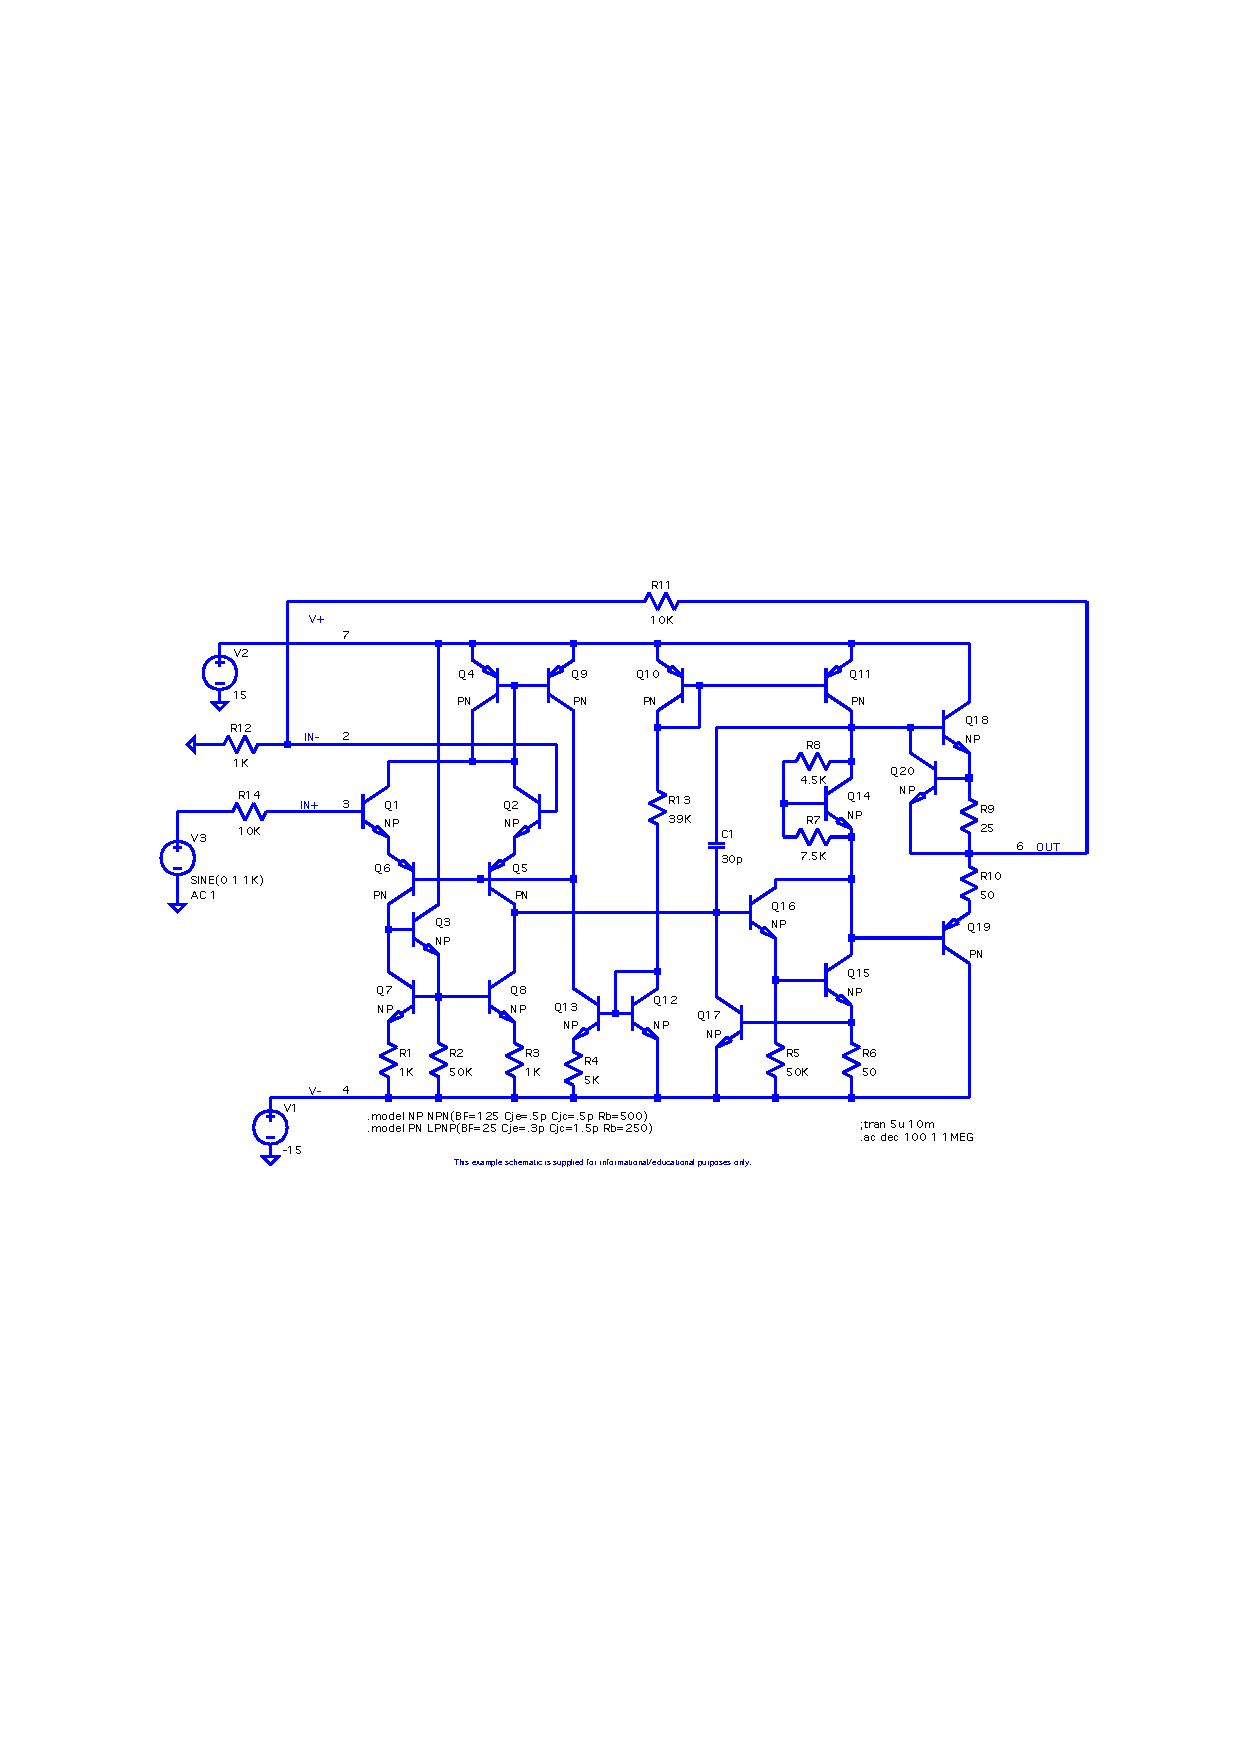
\includegraphics[width=0.8\textwidth]{img/sch_1a.pdf} 
  \caption{Schematic of LM741}
  \label{sch_lm} 
\end{figure}

\begin{figure} [H]
  \centering 
  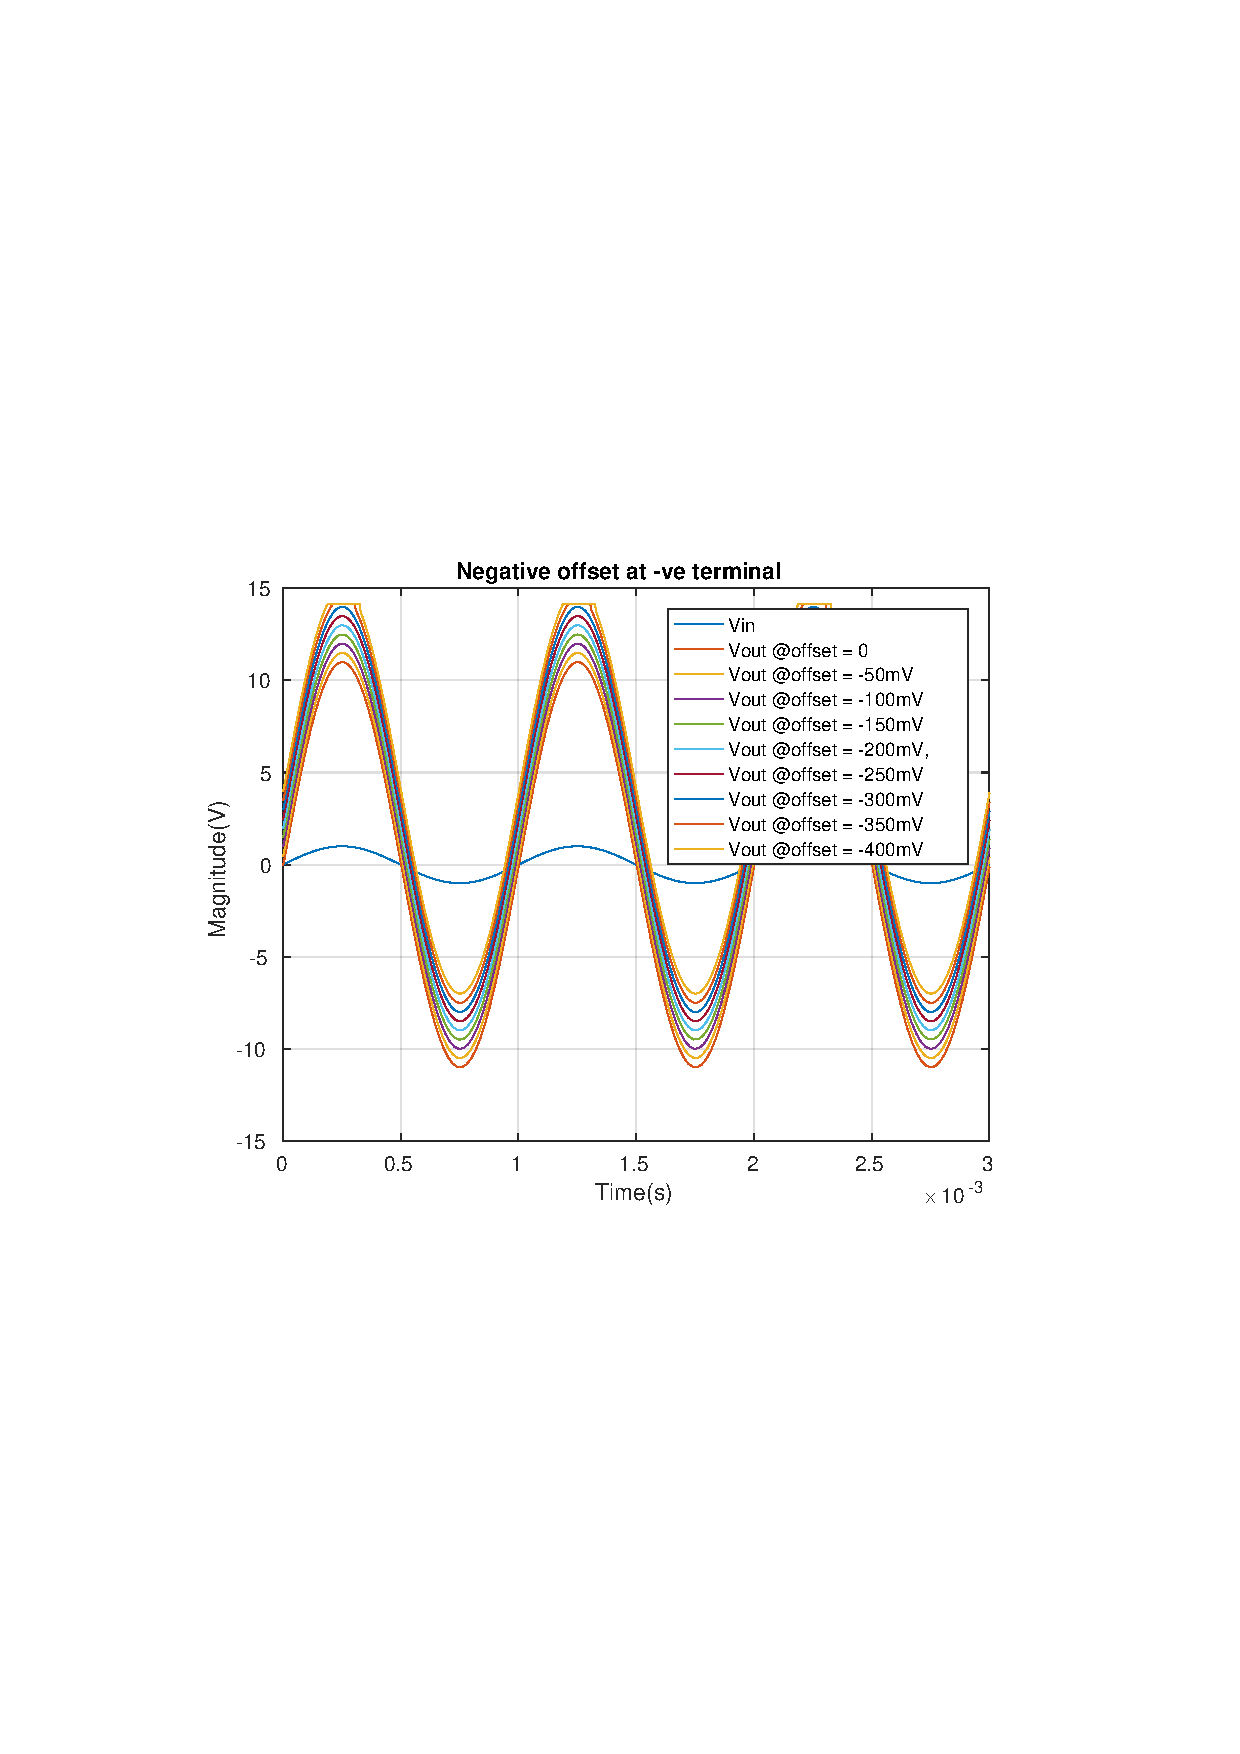
\includegraphics[width=0.8\textwidth]{img/1a_offset_neg.pdf} 
  \caption{Vout with -ve offset at -ve terminal}
  \label{neg_offset} 
\end{figure}

\begin{figure} [H]
  \centering 
  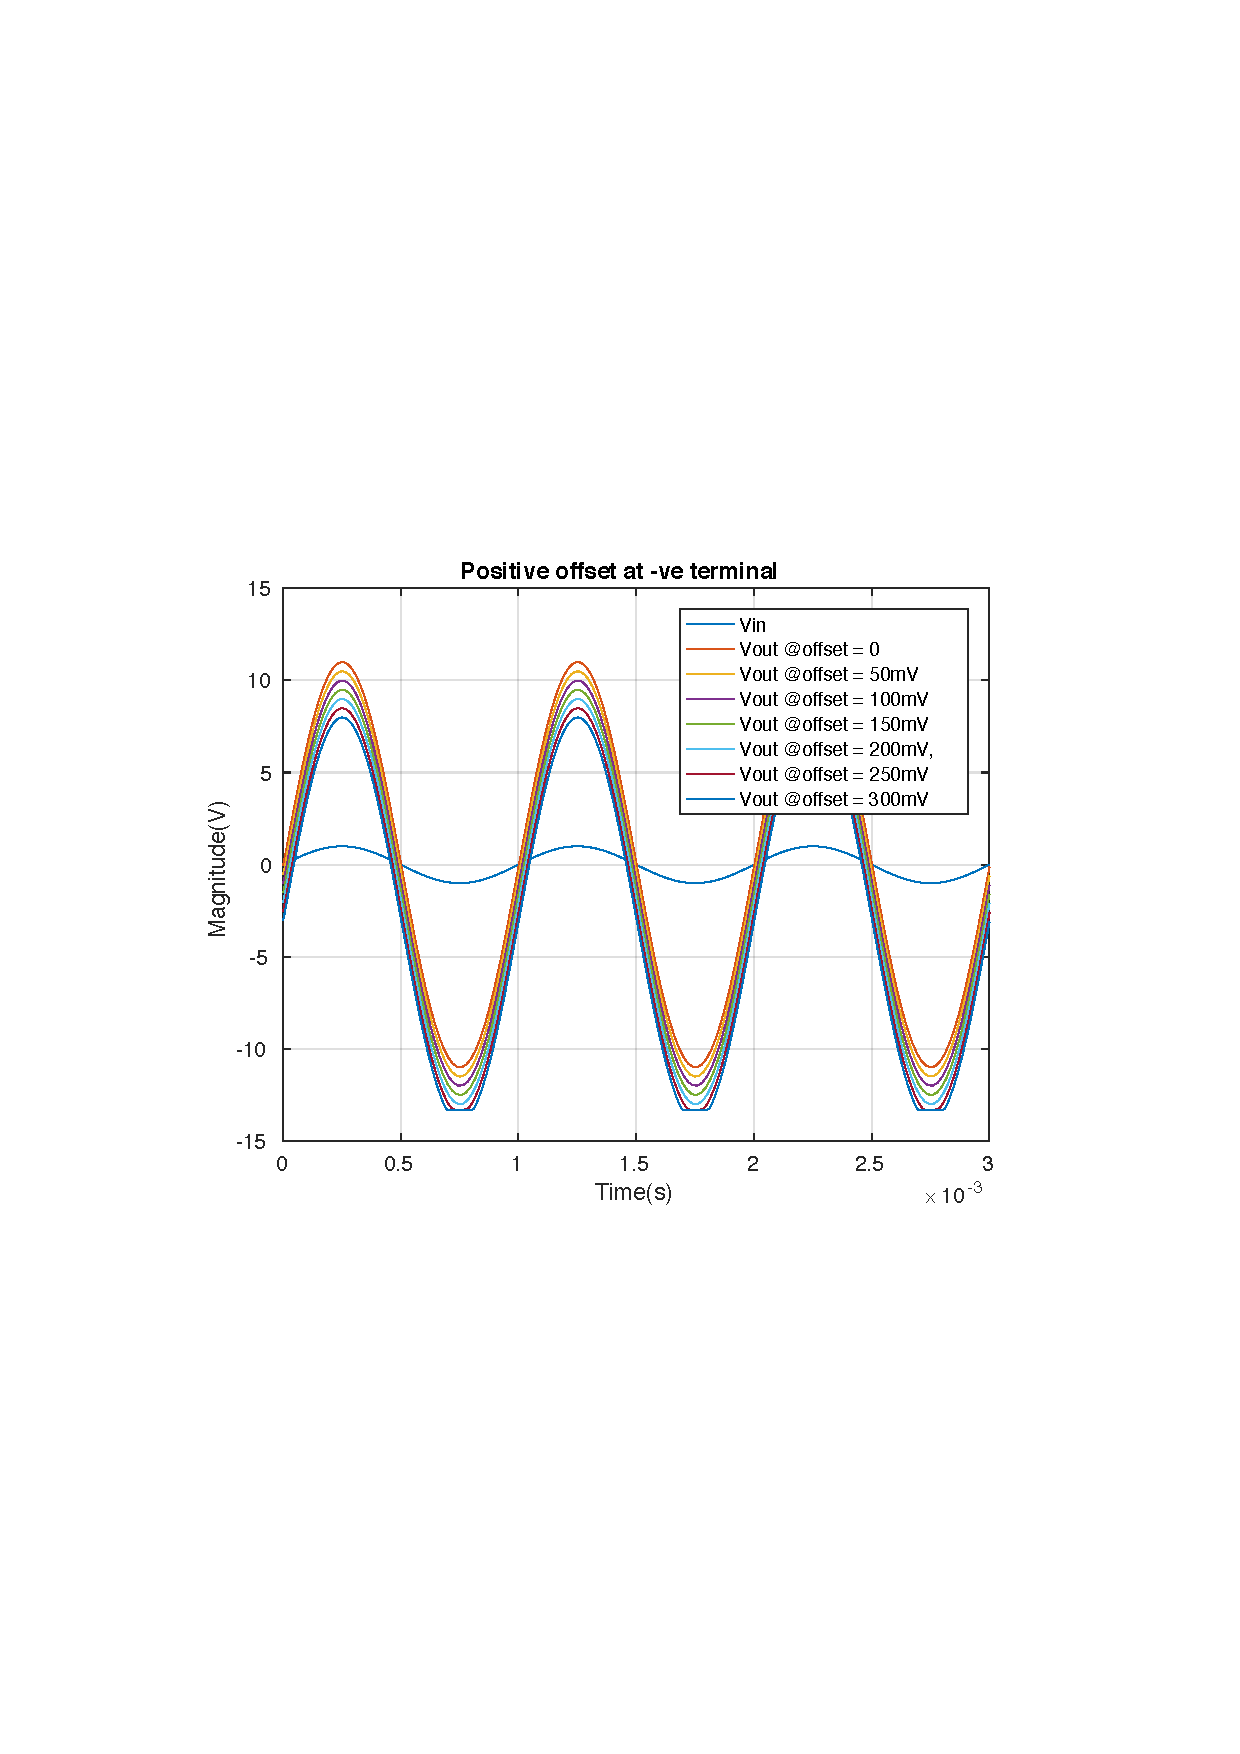
\includegraphics[width=0.8\textwidth]{img/1a_offset_pos.pdf} 
  \caption{Vout with +ve offset at -ve terminal}
  \label{pos_offset} 
\end{figure}

From figure \ref{pos_offset} and \ref{neg_offset}, it is seen that DC-offset interval is -300 mV to 200 mV. When the offset is beyond this interval the ouput saturates to maximum possible output range which is just below +ve and just above -ve supply. This drop in output voltage range is due to the drop in the output stage of amplifier. \\

%% Task 1b
\subsection{AC Analysis}
Figure   \ref{ac_ana}  is the AC analysis of the amplifier. This shows that the DC gain is 20.8 dB and Gain Bandwith(GBW) is 700 KHz. The phase marign(PM) is 95\textdegree (180\textdegree minus phase at 0 dB gain). 

The realtion between DC gain A\textsubscript{v} and GBW is given as 

\begin{equation*}
GBW = A_v*BW
\end{equation*}
where BW is -3dB bandwidth.
\begin{figure} [H]
  \centering 
  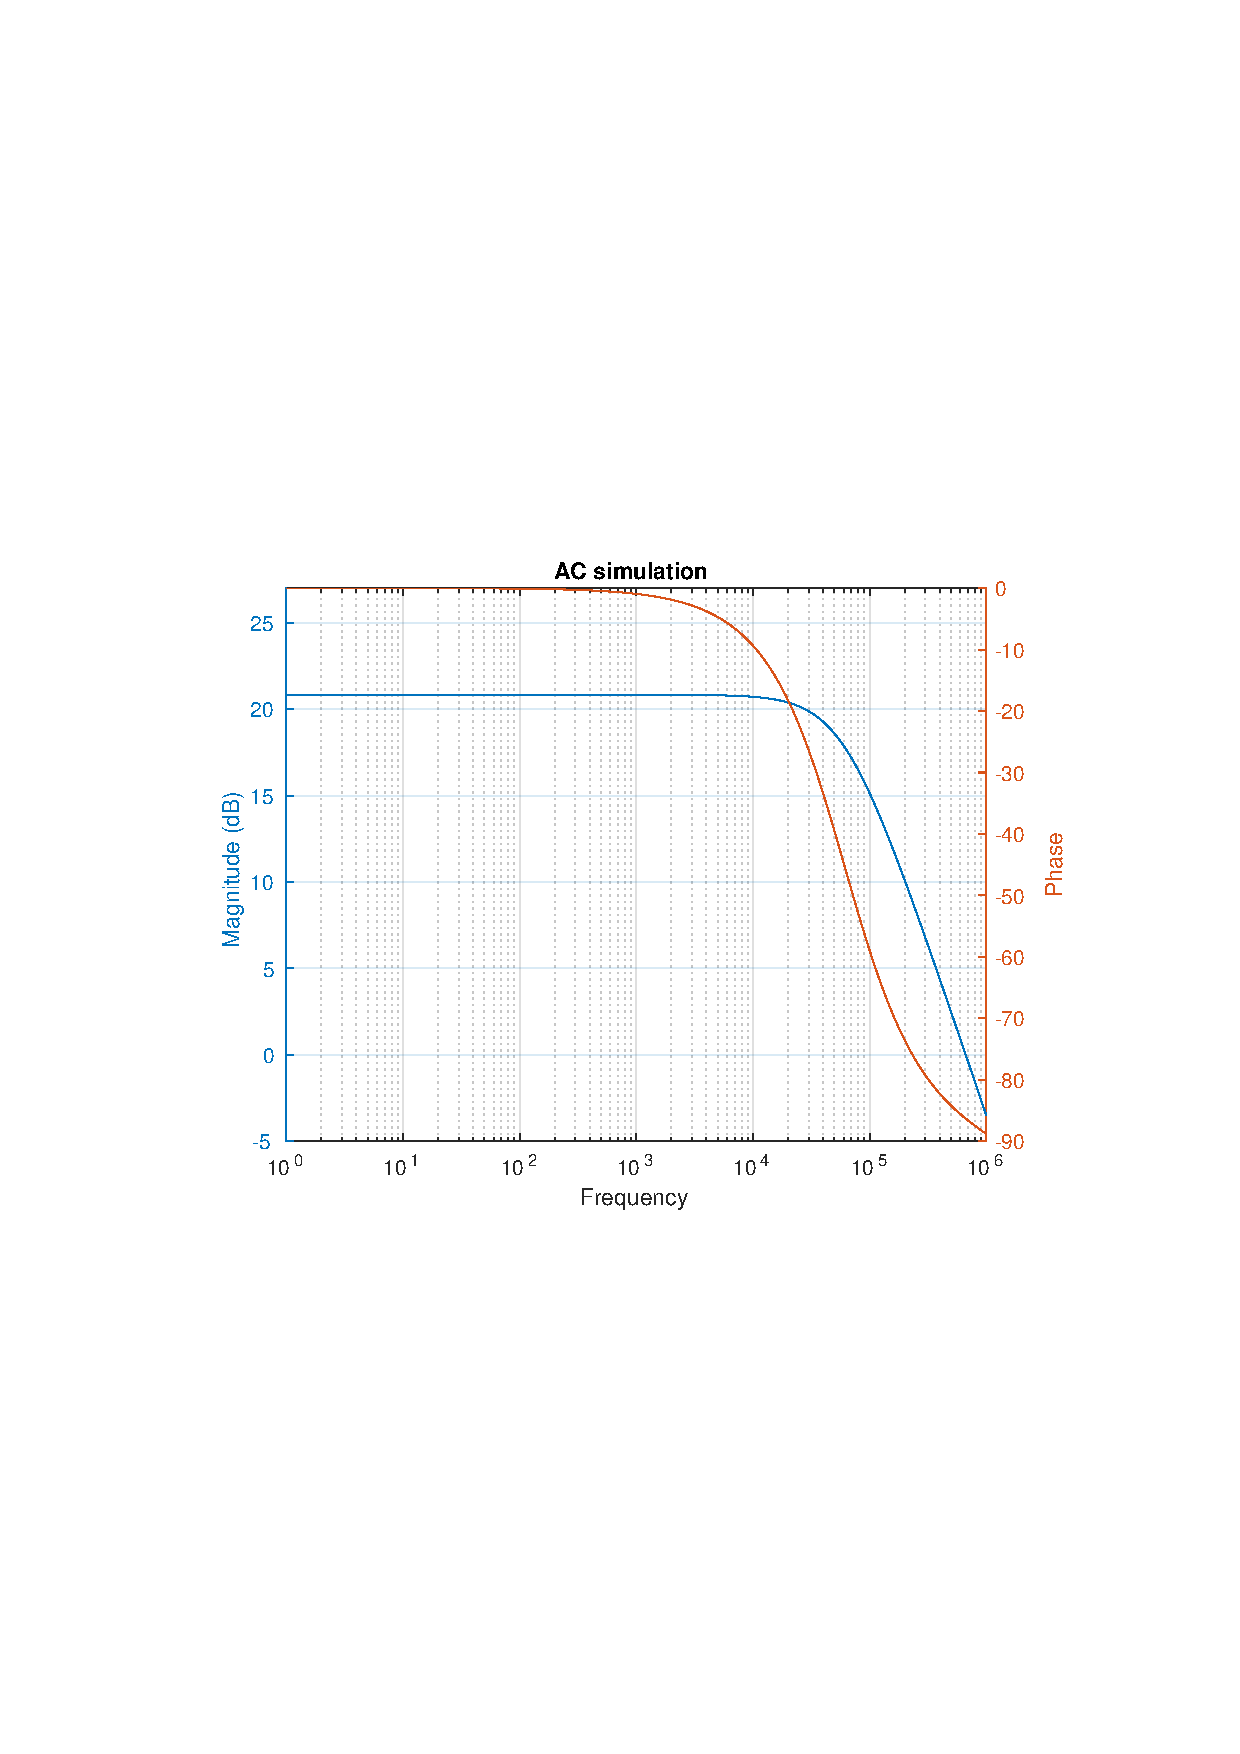
\includegraphics[width=0.9\textwidth]{img/1b.pdf} 
  \caption{AC analysis of given opamp}
  \label{ac_ana} 
\end{figure}

%% Task 1c
\subsection{DC-offset}
Figure  \ref{ac_pos}  shows the variation of DC gain for different +ve common mode (CM) voltages. Only the DC CM levels where the gain decreases are shown. It is seen from the plot that for DC CM of 14.992 V or less, the DC gain is at -6 dB or greater.

Similarly  \ref{ac_neg} shows the -ve DC CM where the gain  decreases. It shows that for DC CM of -12.847 V or more, the DC gain is -6 dB or greater. It can be said that the minus terminal DC range of the amplifier is -12.847 V to 14.992 V where the gain is within -6 dB.

\begin{figure} [H]
  \centering 
  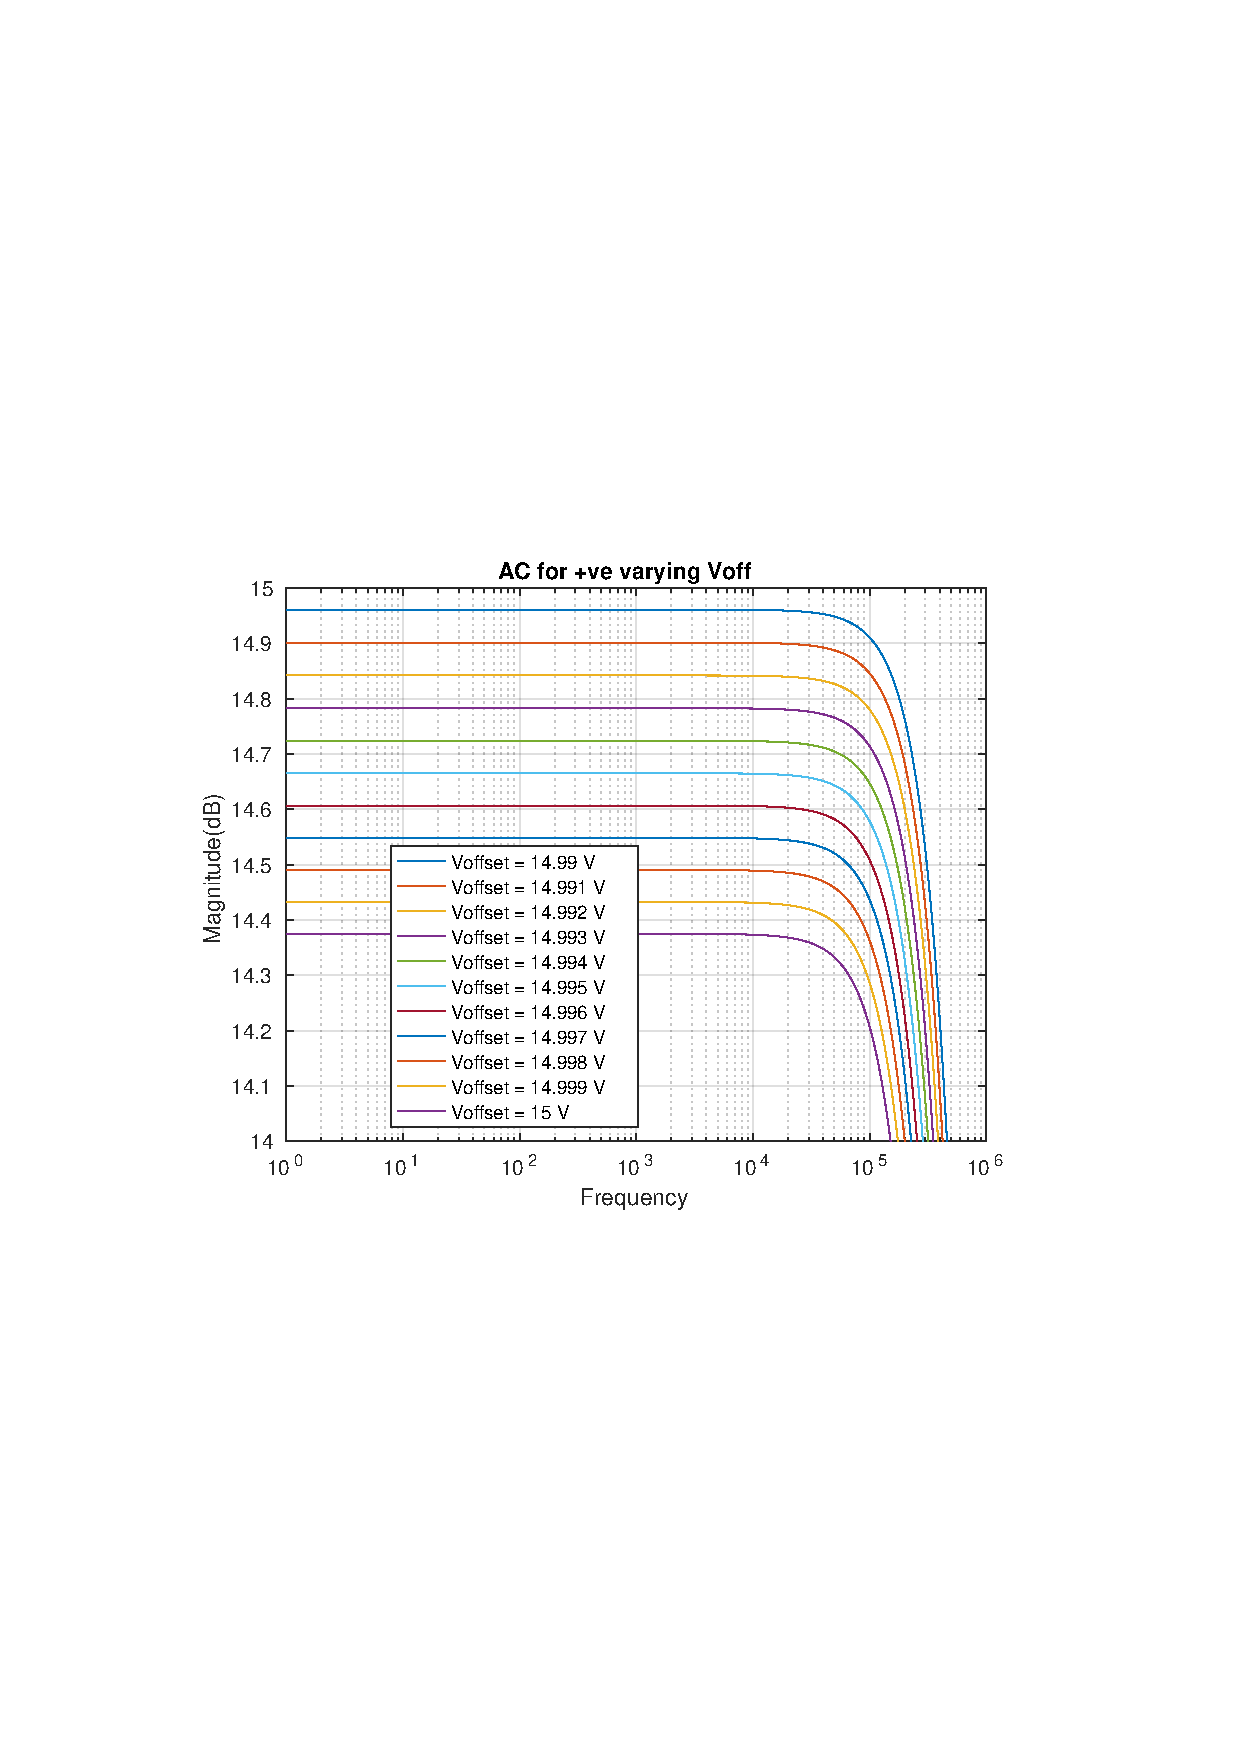
\includegraphics[width=0.8\textwidth]{img/1c_pos_offset.pdf} 
  \caption{AC analysis with varying +ve offset}
  \label{ac_pos} 
\end{figure}

\begin{figure} [H]
  \centering 
  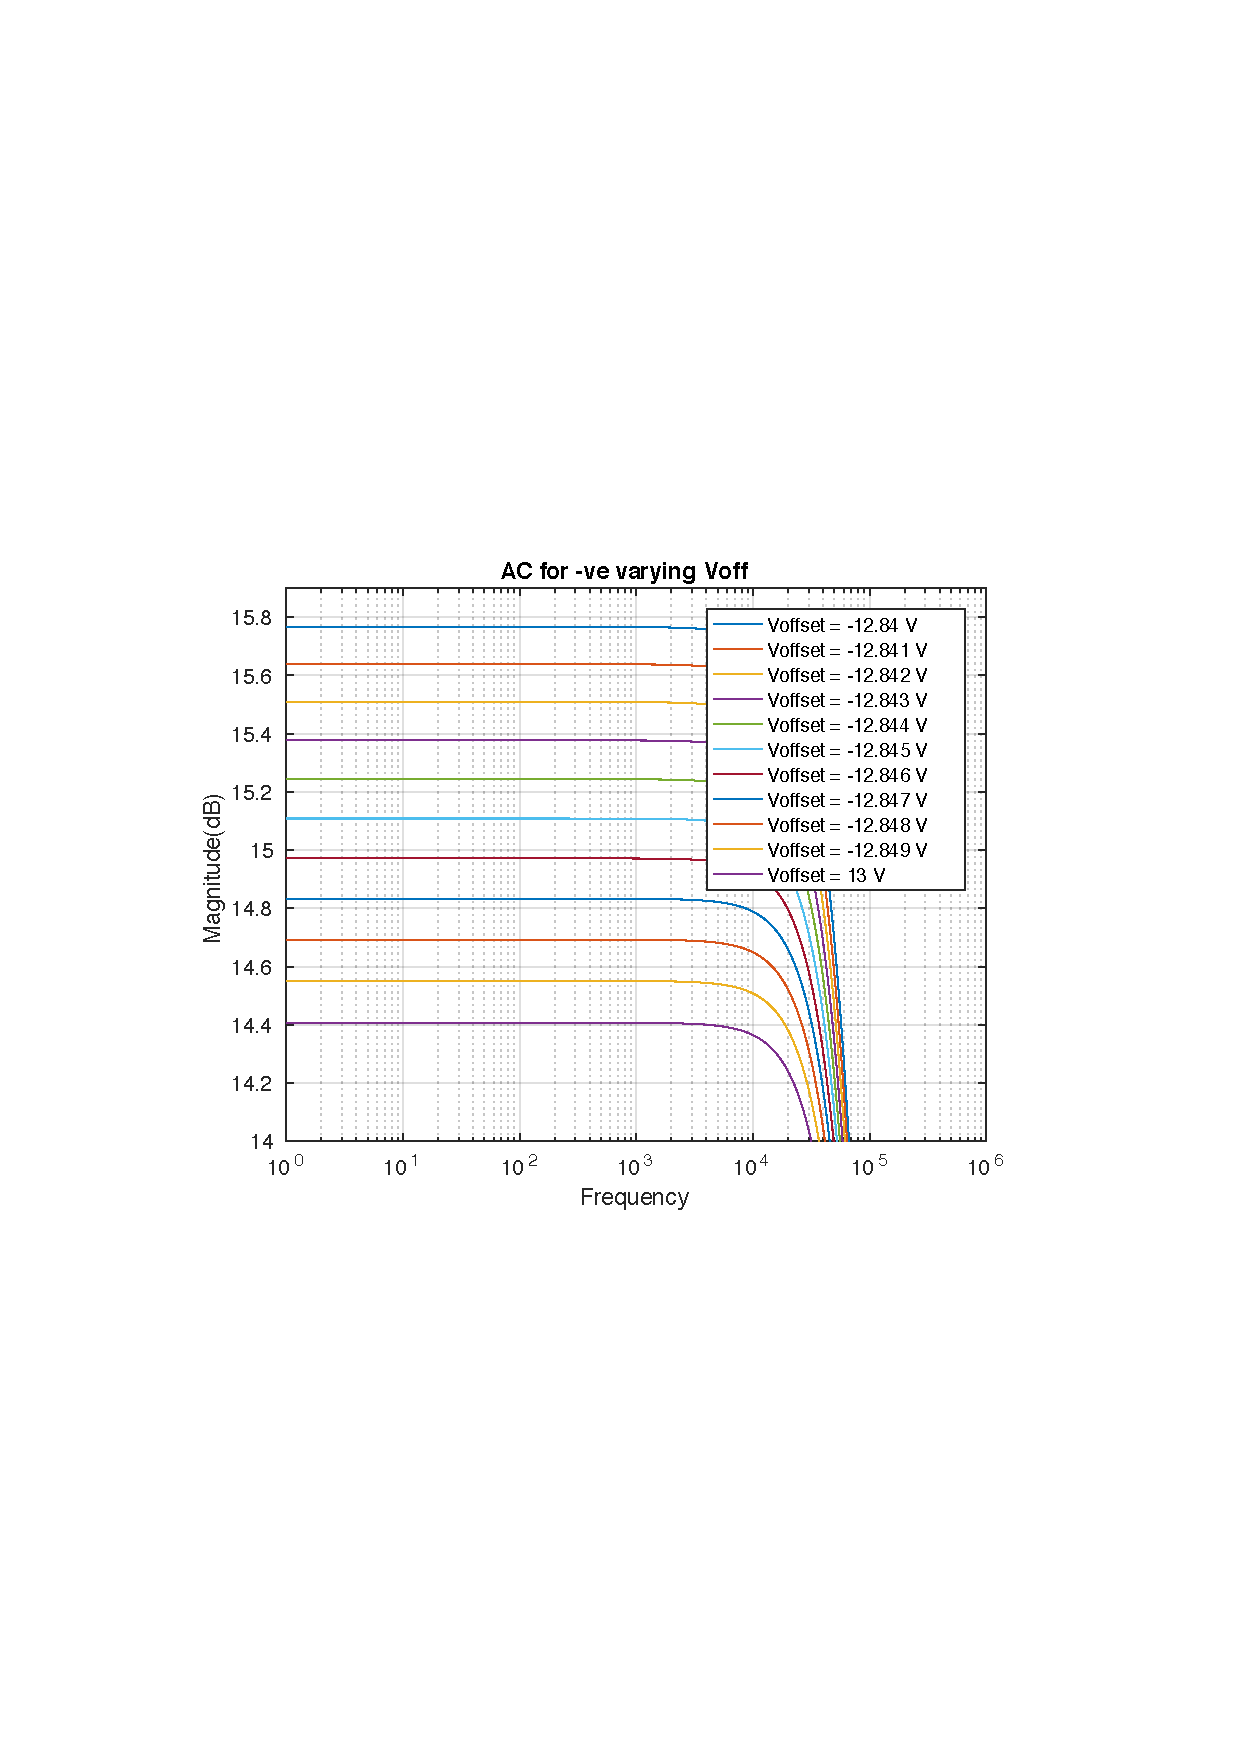
\includegraphics[width=0.8\textwidth]{img/1c_neg_offset.pdf} 
  \caption{AC analysis with varying -ve offset}
  \label{ac_neg} 
\end{figure}

%% Task 1d
\subsection{Load capacitance }
 Figure \ref{sch_1d}  is schematic and figure \ref{ac_cload} is  result of  AC simulation with C\textsubscript{load} step of 10pF from 10pF to 30pF. The plot shows that increase in load capacitor has significantly affected the phase by increasing it whereas the gain remains almost constant. This means PM has decreased. 
\begin{figure} [H]
  \centering 
  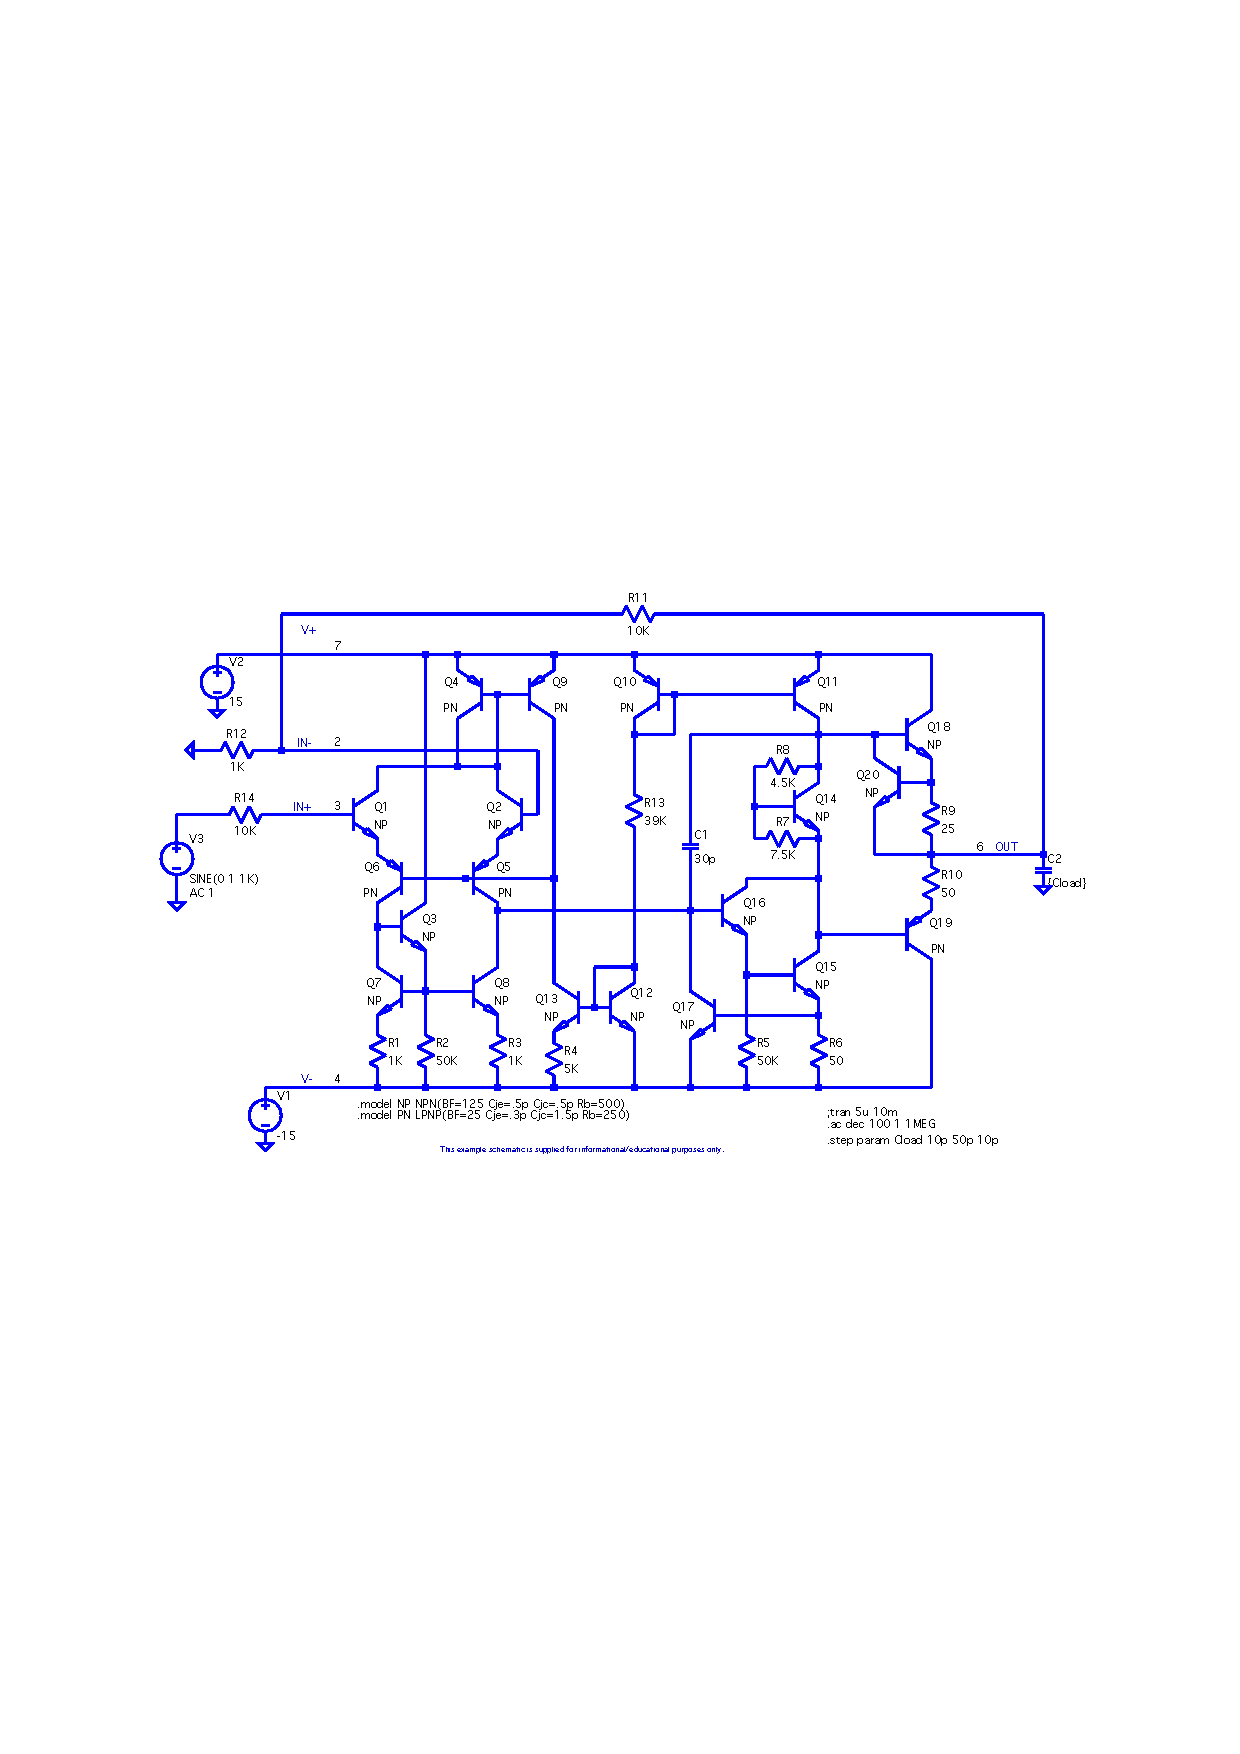
\includegraphics[width=0.75\textwidth]{img/sch_1d.pdf} 
  \caption{Schematic setup for ac simulation}
  \label{sch_1d} 
\end{figure}


\begin{figure} [H]
  \centering 
  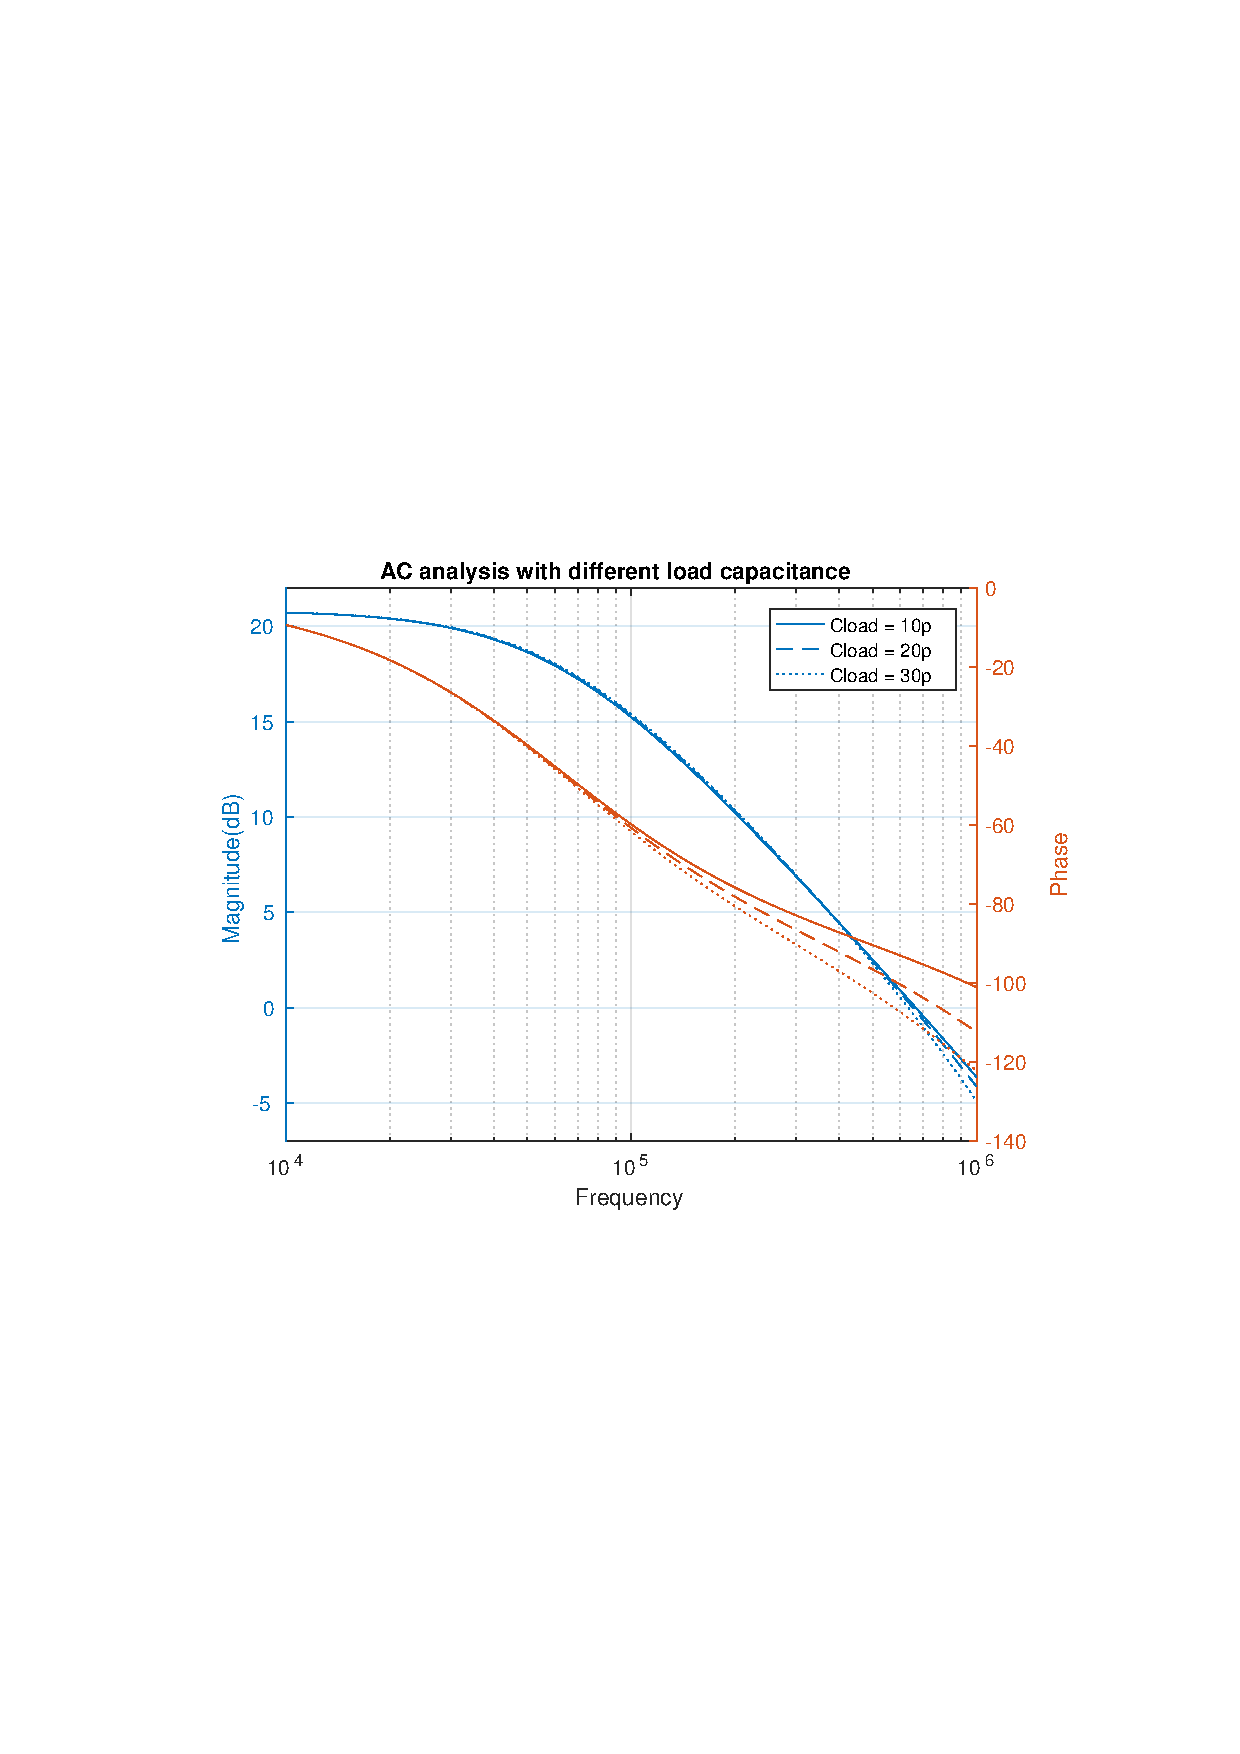
\includegraphics[width=0.8\textwidth]{img/1d.pdf} 
  \caption{AC analysis with different load capacitance}
  \label{ac_cload} 
\end{figure}

%% Task 2
\section{Frequency characteristics of some curves}
%% Task 2a
\subsection{FFT with different sampling rates}

A low pass (LP) RC filter is deigned. R and C values are arbitrarily chosen $1 \Omega$ and $1pF$ respectively so that it has a very high cutoff frequency. 

A sine wave signal of period 1 ms and amplitude 1 V, as shown in figure \ref{tran_sin}, is applied at the input of the filter. This transient signal was sampled at 1/10 and 1/100 of the period and their corresponding FFT was done as shown in \ref{fft_sin}. FFT clearly shows how different sampling rates affects the frequency components of the same signal. Since a pure sine wave has only one frequency component, it is expected to see only it natural frequency in FFT. But figure  \ref{fft_sin} shows the harmonics too. It is because the sampled data of true sine wave is in-fact not representing it truly because of lower sampling rate. The strength of  strongest unwanted frequency component is -40 dB.  It can be concluded that the sampling rate of the measuring device actually affects the frequency components of signal. Instrument with low sampling frequency can give us misleading informations.

\begin{figure} [H]
  \centering 
  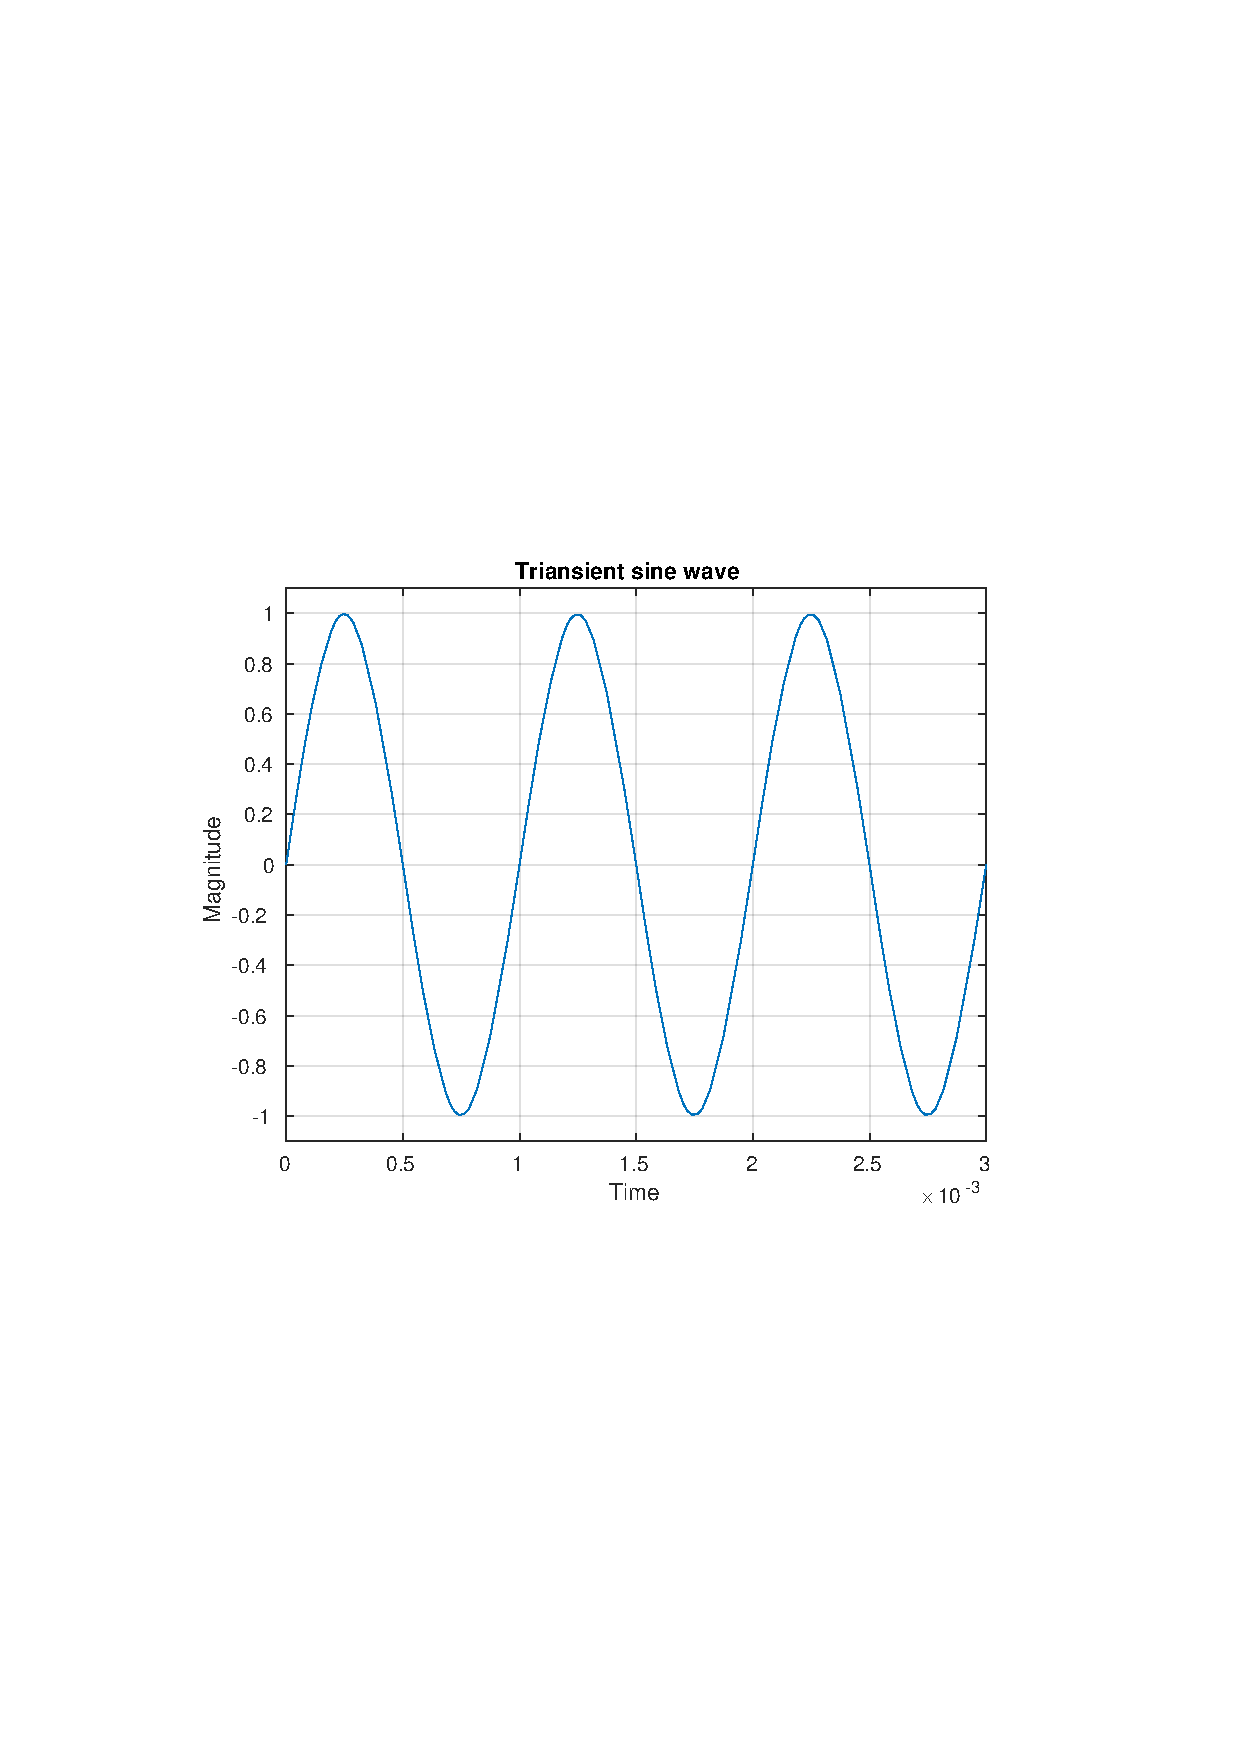
\includegraphics[width=0.8\textwidth]{img/2a_tran.pdf} 
  \caption{Sine wave}
  \label{tran_sin} 
\end{figure}

\begin{figure} [H]
  \centering 
  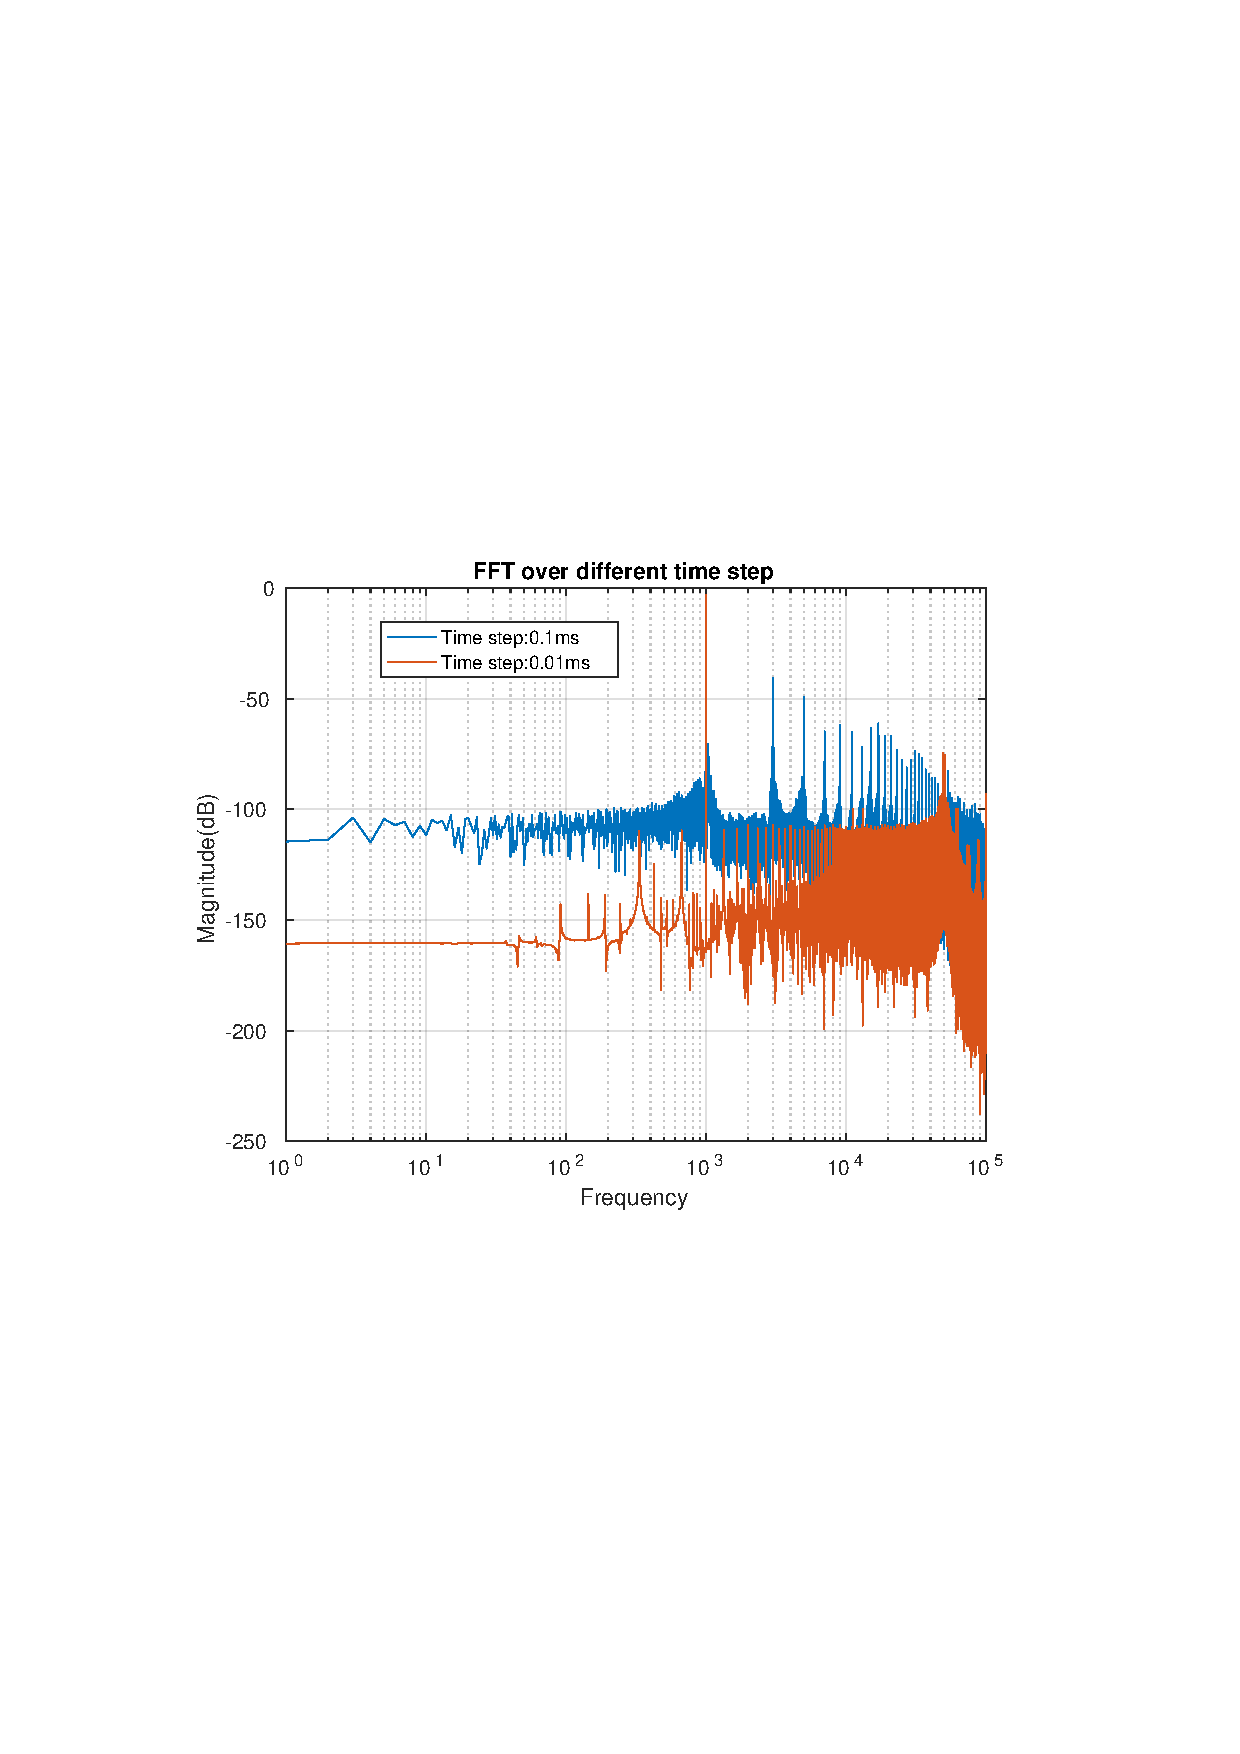
\includegraphics[width=0.9\textwidth]{img/2a.pdf} 
  \caption{FFT of \ref{tran_sin} with different time step}
  \label{fft_sin} 
\end{figure}


%% Task 2b
\subsection{FFT of signals with different falling (T\textsubscript{f}) and rising (T\textsubscript{r}) time}
Figure \ref{tran_all} shows three different signals with same frequency but with different rising and falling time. FFT of all signals were performed and their respective frequency components were obtained as illustrated by figure \ref{fft_all}. It is seen that a triangular signal which has longer falling and rising time has dominant low frequency components but sharply falling higher frequency components. Similarly when the signal is square like with shorter rise and fall time, it has prominent higher frequency component. 

The strongest fundamental frequency is 1KHz which has magnitude if -8 dB.

The clock edge should look like ramp like that of triangle pulse in order to reduce the high frequency component in the signal. However having a ramp with gently sloping edge reduces the speed of CMOS logic. Moreover the ON and OFF period may not be properly defined. 

\begin{figure} [H]
  \centering 
  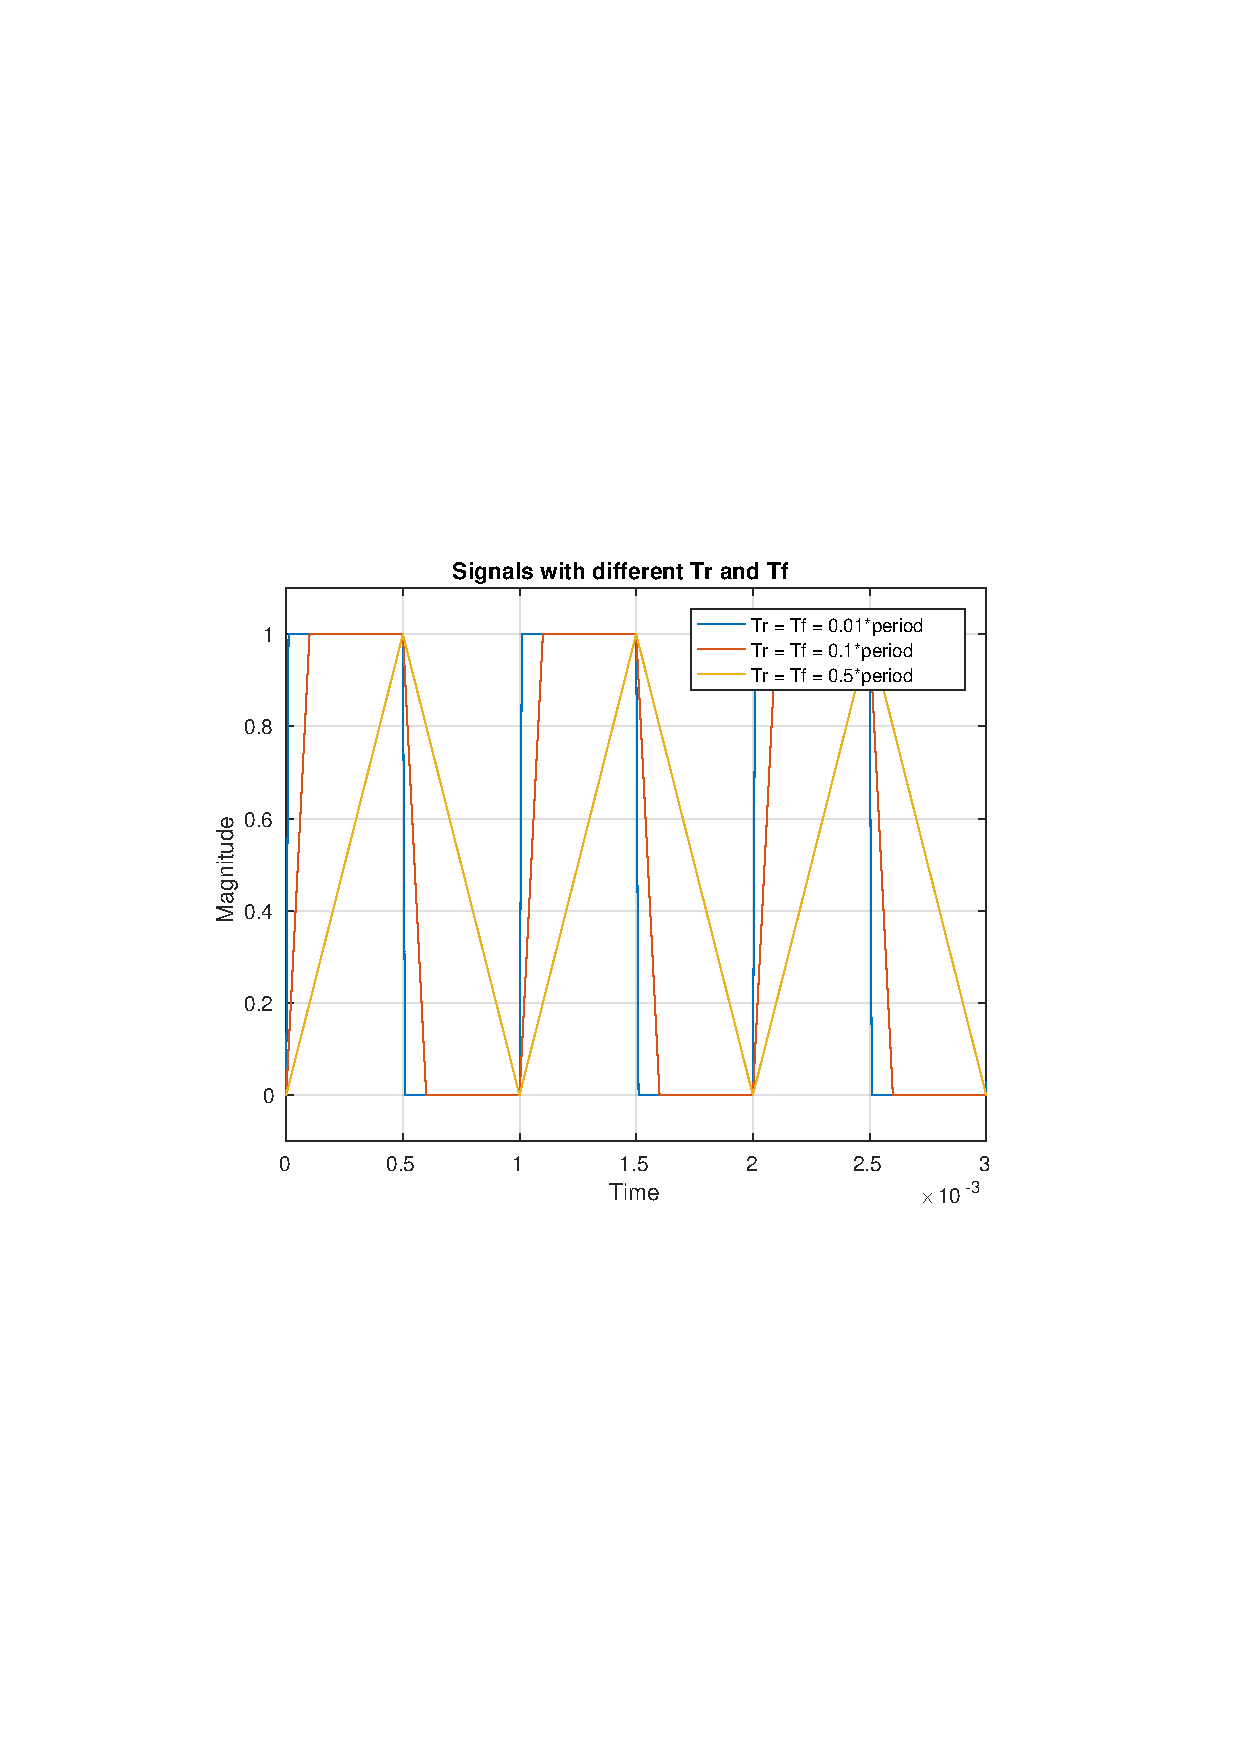
\includegraphics[width=0.8\textwidth]{img/2b_tran.pdf} 
  \caption{Signals with different rise and fall time}
  \label{tran_all} 
\end{figure}

\begin{figure} [H]
  \centering 
  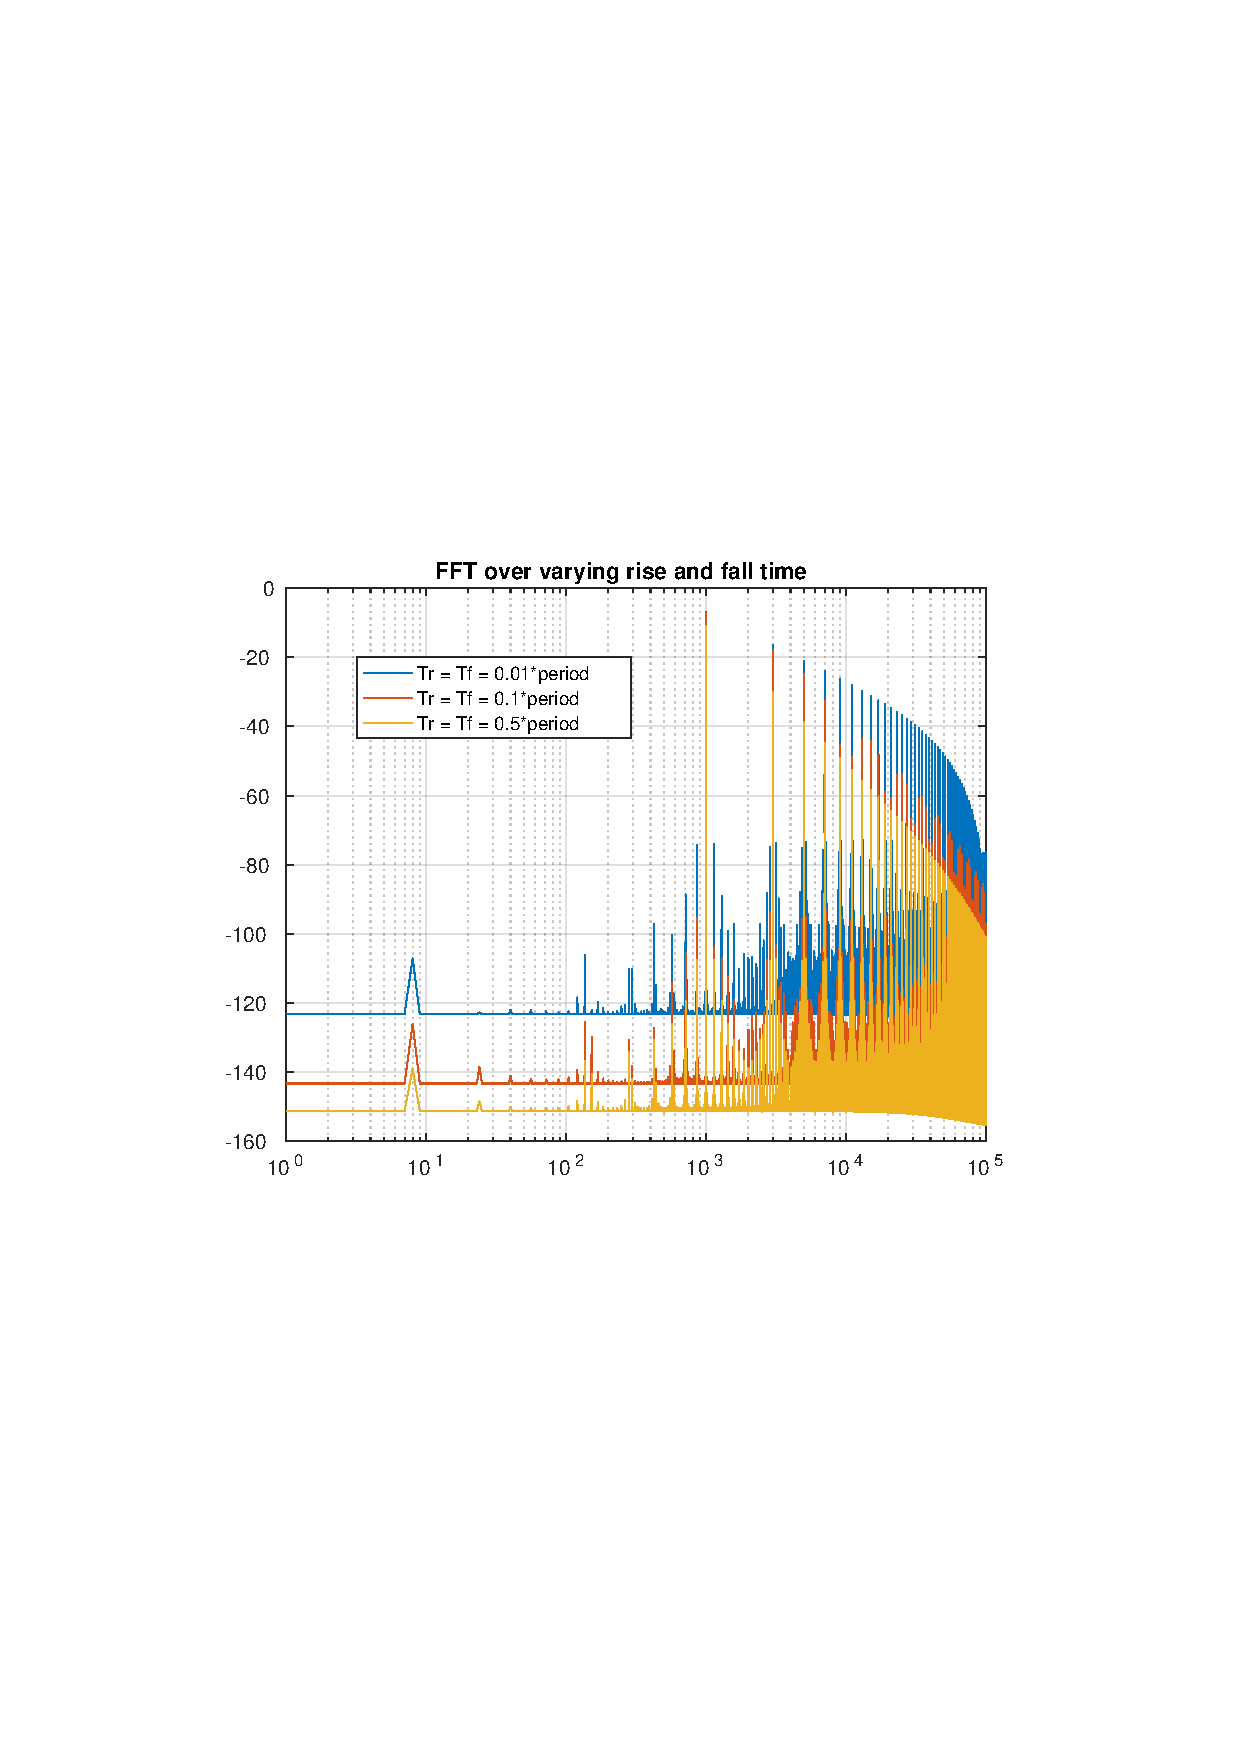
\includegraphics[width=0.8\textwidth]{img/2b_fft.pdf} 
  \caption{FFT of \ref{tran_all} signals}
  \label{fft_all} 
\end{figure}


%% Task 2c
\subsection{RC filter}
RC filter shown in figure above is made to have cutoff at 5 times its natural frequency, ie 5 kHz. R and C values were obtained to be 1K and 25nF respectively. Square wave with frequency 1 KHz with rise and fall time of 1/100 of its period  was applied as input and its output was observed as shown in figure \ref{tran_tuned}.
FFT of the both the input and output was done as in figure \ref{fft_tuned}. The output signal has longer rise and fall time because of larger capacitor at the output. which means output has more low frequency components than the input which is clearly shown by the FFT plot.

\begin{figure} [H]
  \centering 
  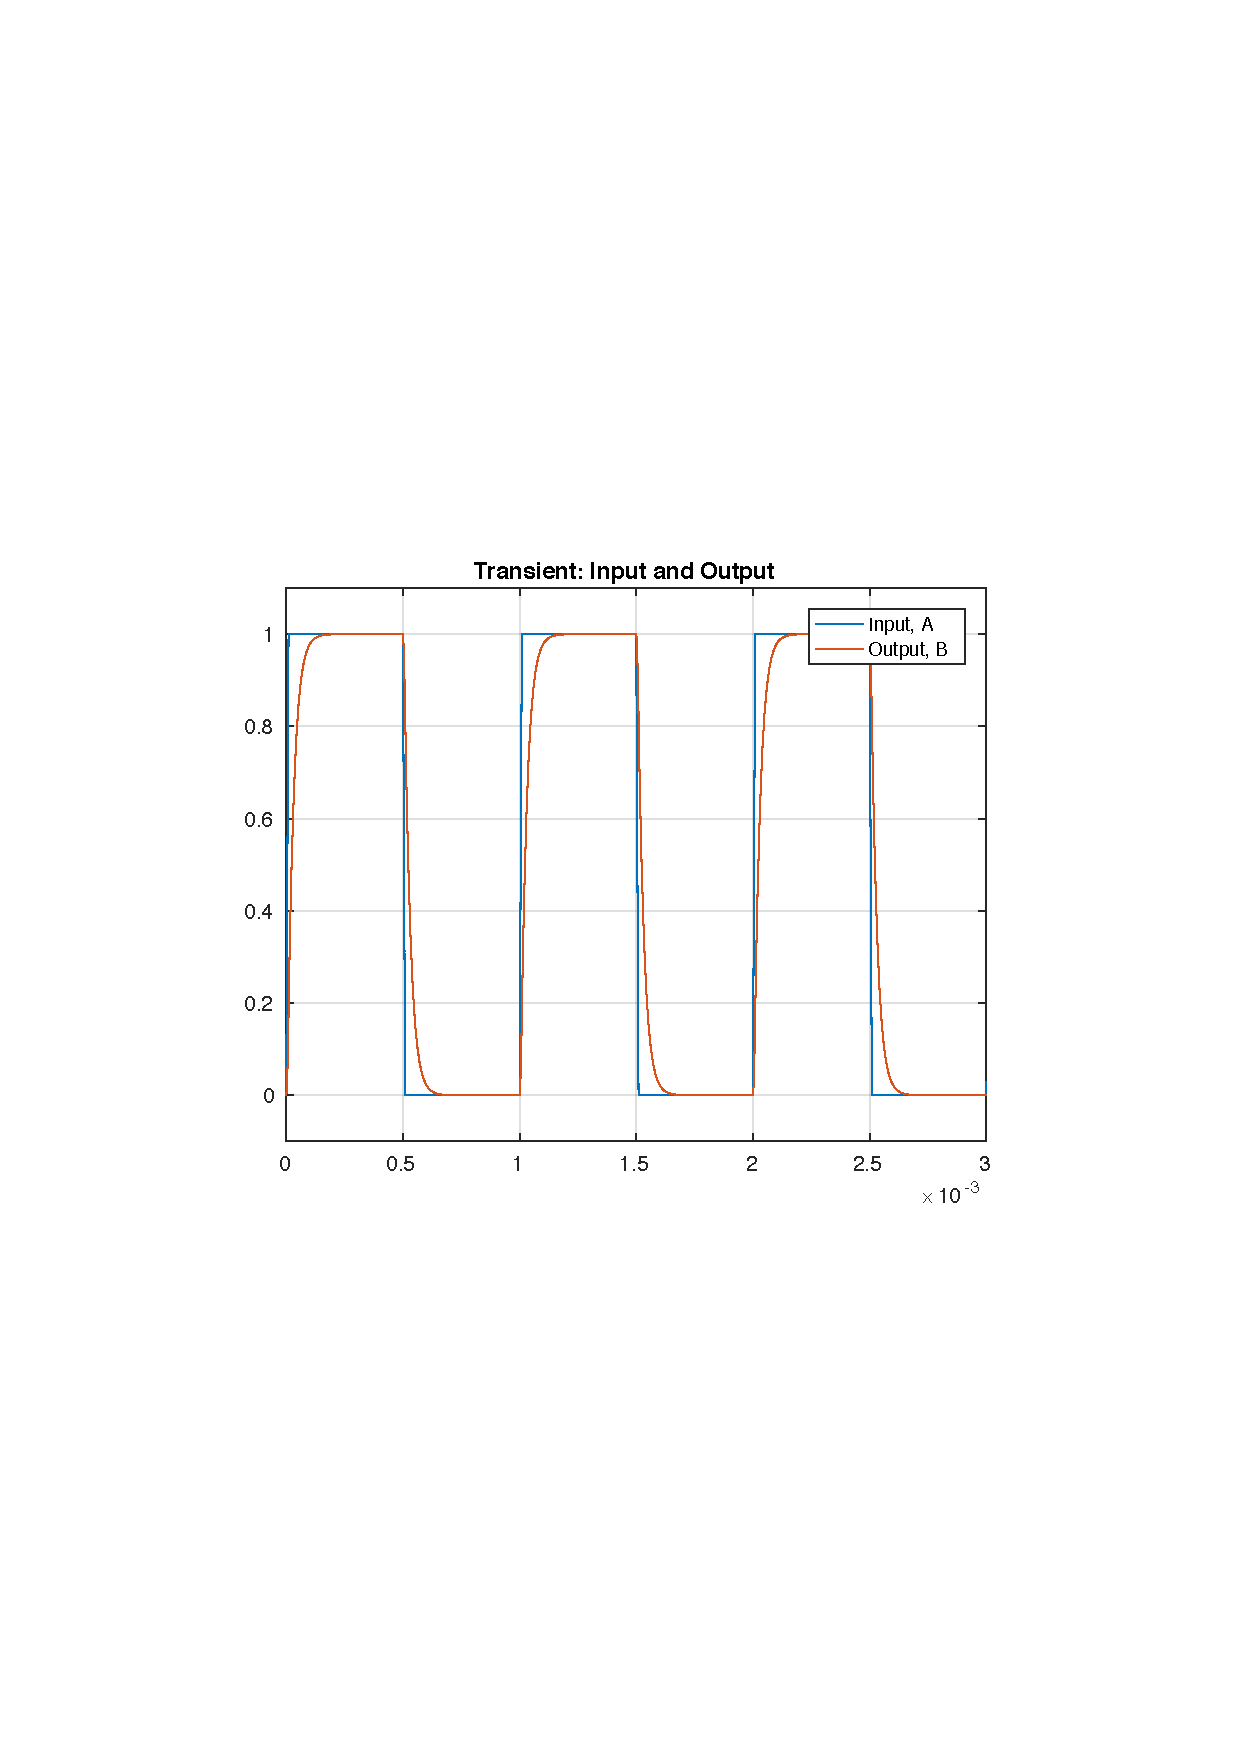
\includegraphics[width=0.9\textwidth]{img/2c_tran.pdf} 
  \caption{Input and output of LP filter}
  \label{tran_tuned} 
\end{figure}

\begin{figure} [H]
  \centering 
  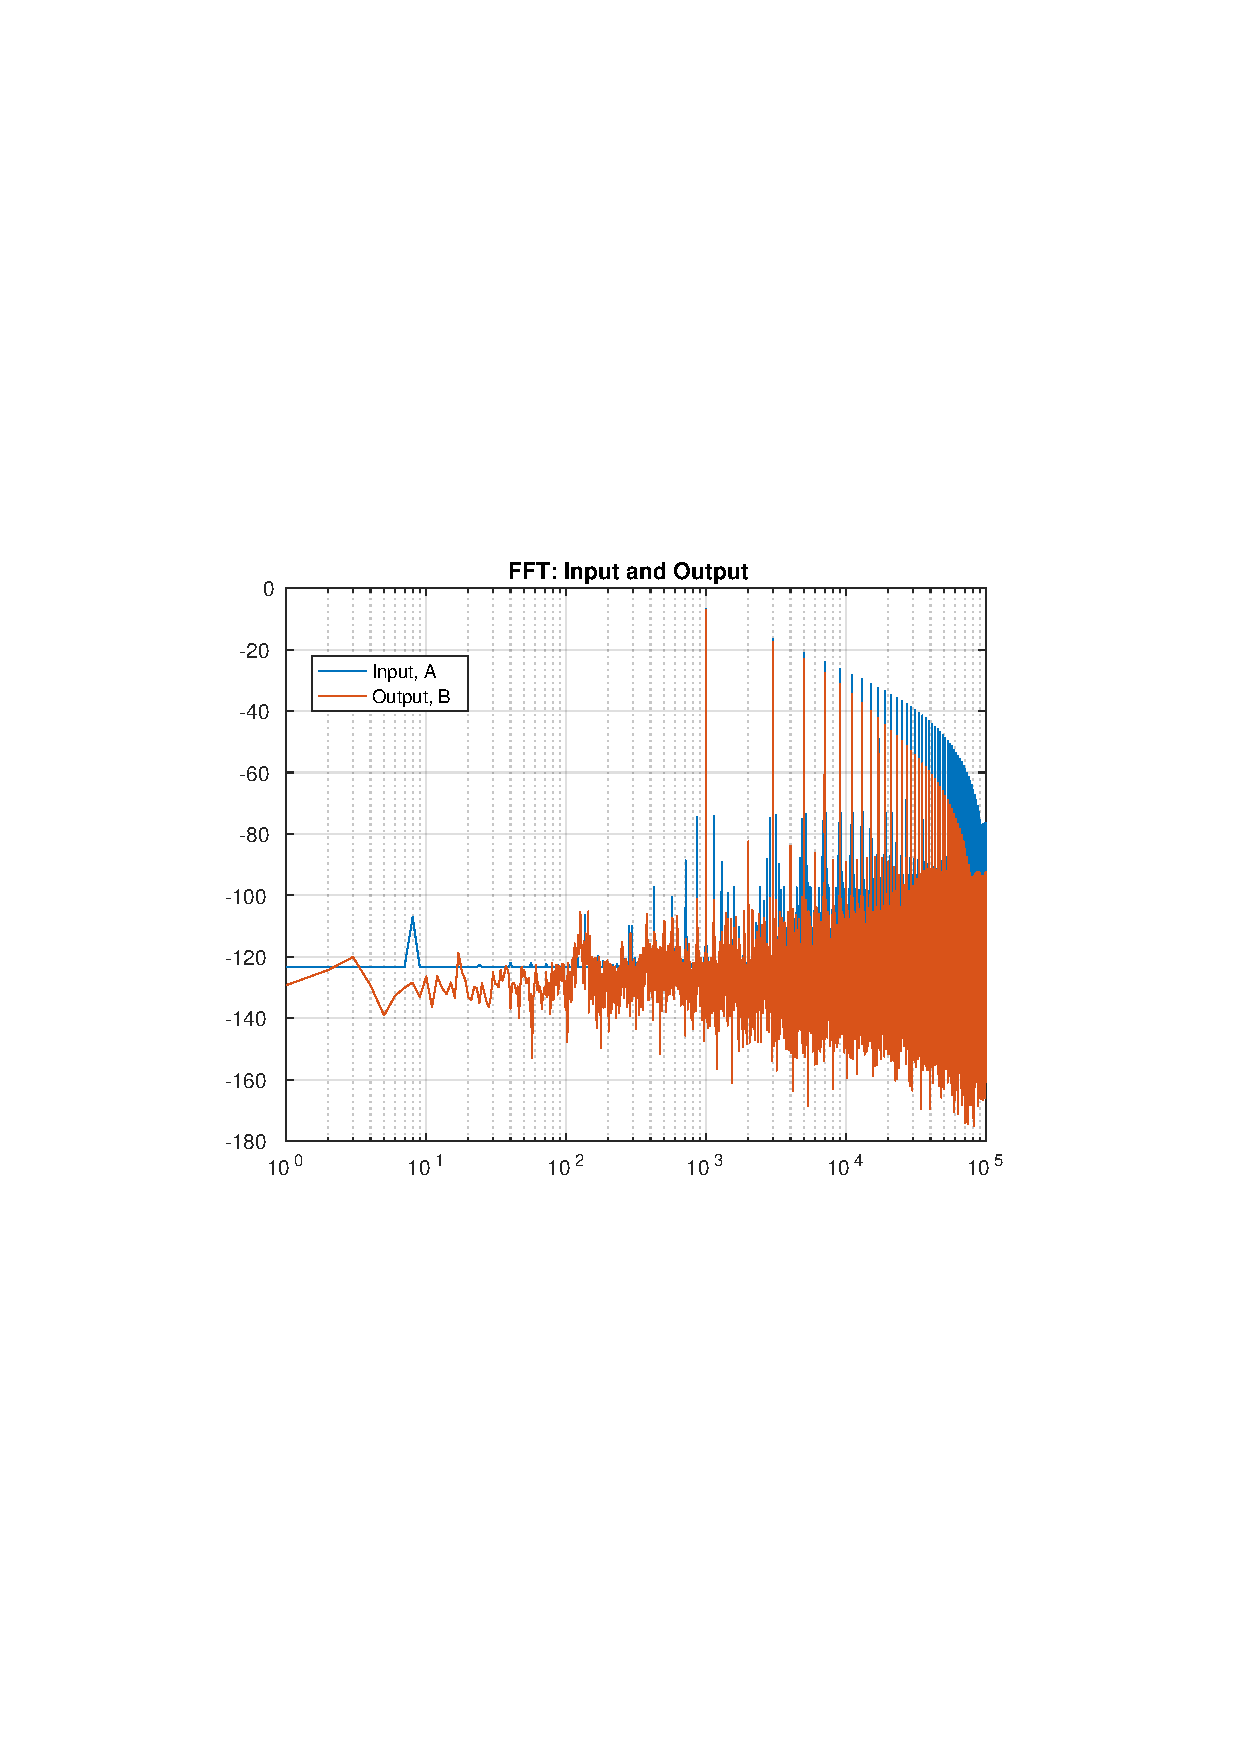
\includegraphics[width=0.9\textwidth]{img/2c_fft.pdf} 
  \caption{FFT of \ref{tran_tuned} signals}
  \label{fft_tuned} 
\end{figure}

%% Task 3
\section{Decoupling capacitors}
Given in the question that $L = 10 nH$ for each capacitor, current spikes (triangular wave) of 0-1 A amplitude with $T_r = T_f = 5 ns$, $Ton = 0$, period = 10 us, voltage at the output to be stable within 5\% of 1.5 V and lower corner frequency at 1MHz. 
%% Task 3a
\subsection{}
Low frequency target impedance, $Z_t= k dV/dI$ is given as
\begin{equation*}
Z_t= k \frac{dV}{dI}
\end{equation*}
 where $k = 2$, $dV = 0.075 V$ and $dI = 1 A$. Hence $Z_t = 0.15 \Omega$.
%% Task 3b
\subsection{}
Number of capacitors required is given as
\begin{equation*}
n =  \frac{2L}{Z_tT_r}
\end{equation*}
where $L = 10nH$, $T_r = 5 ns$. Hence $n = 27$. Then each inductor has inductance  $370 pH (L/n)$.
%% Task 3c
\subsection{}
The total capacitance is given by the condition
\begin{eqnarray*}
\frac{1}{\omega C}& \leq & Z_t  \\
C  &  \geq&\frac{1}{2\pi f Z_t}
\end{eqnarray*}
where $f=1 MHz$. Hence, $ C = 1.1 uF$ and hence each capacitor is 40 nF.
%% Task 3d
\subsection{}
The high frequency corner decided by rise/fall time is given as 
\begin{equation*}
f = \frac{1}{\pi*T_r}
\end{equation*}
Hence is $f=64 MHz$.
%% Task 3e
\subsection{}
Figure \ref{sch_3} is the schematic and figure  \ref{cap_tran} and  \ref{cap_ac}  are transient and frequency simulation results. In the transient simulation, the voltage spikes due to the current spikes can be seen. The voltage spikes are between 40 mV to -55 mV,  well below the requirement.

Similarly from the ac simulation, the lower and upper corner frequency can be noticed around 1 MHz and 64 MHz as calculated.

\begin{figure} [H]
  \centering 
  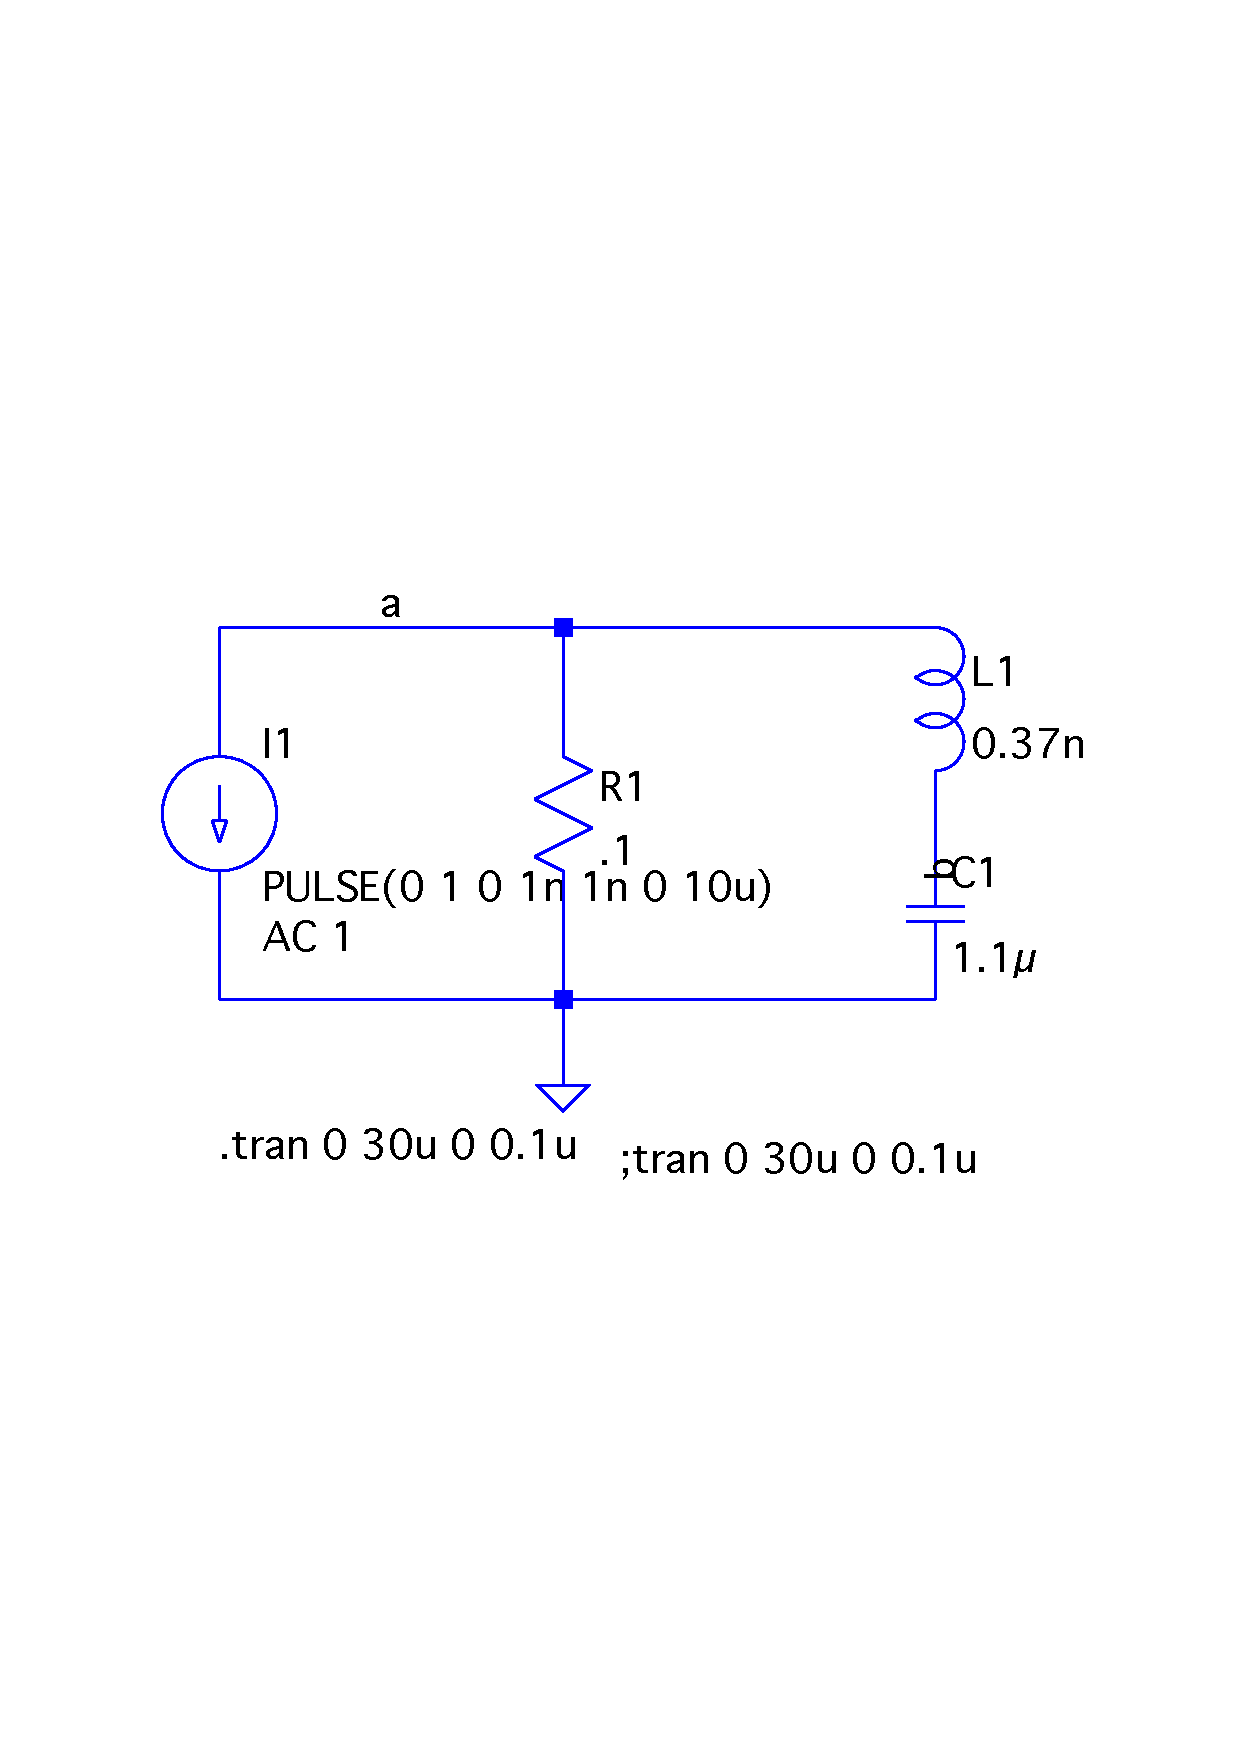
\includegraphics[width=0.8\textwidth]{img/sch_3.pdf} 
  \caption{Schematic set up of a single decoupling capacitor}
  \label{sch_3} 
\end{figure}


\begin{figure} [H]
  \centering 
  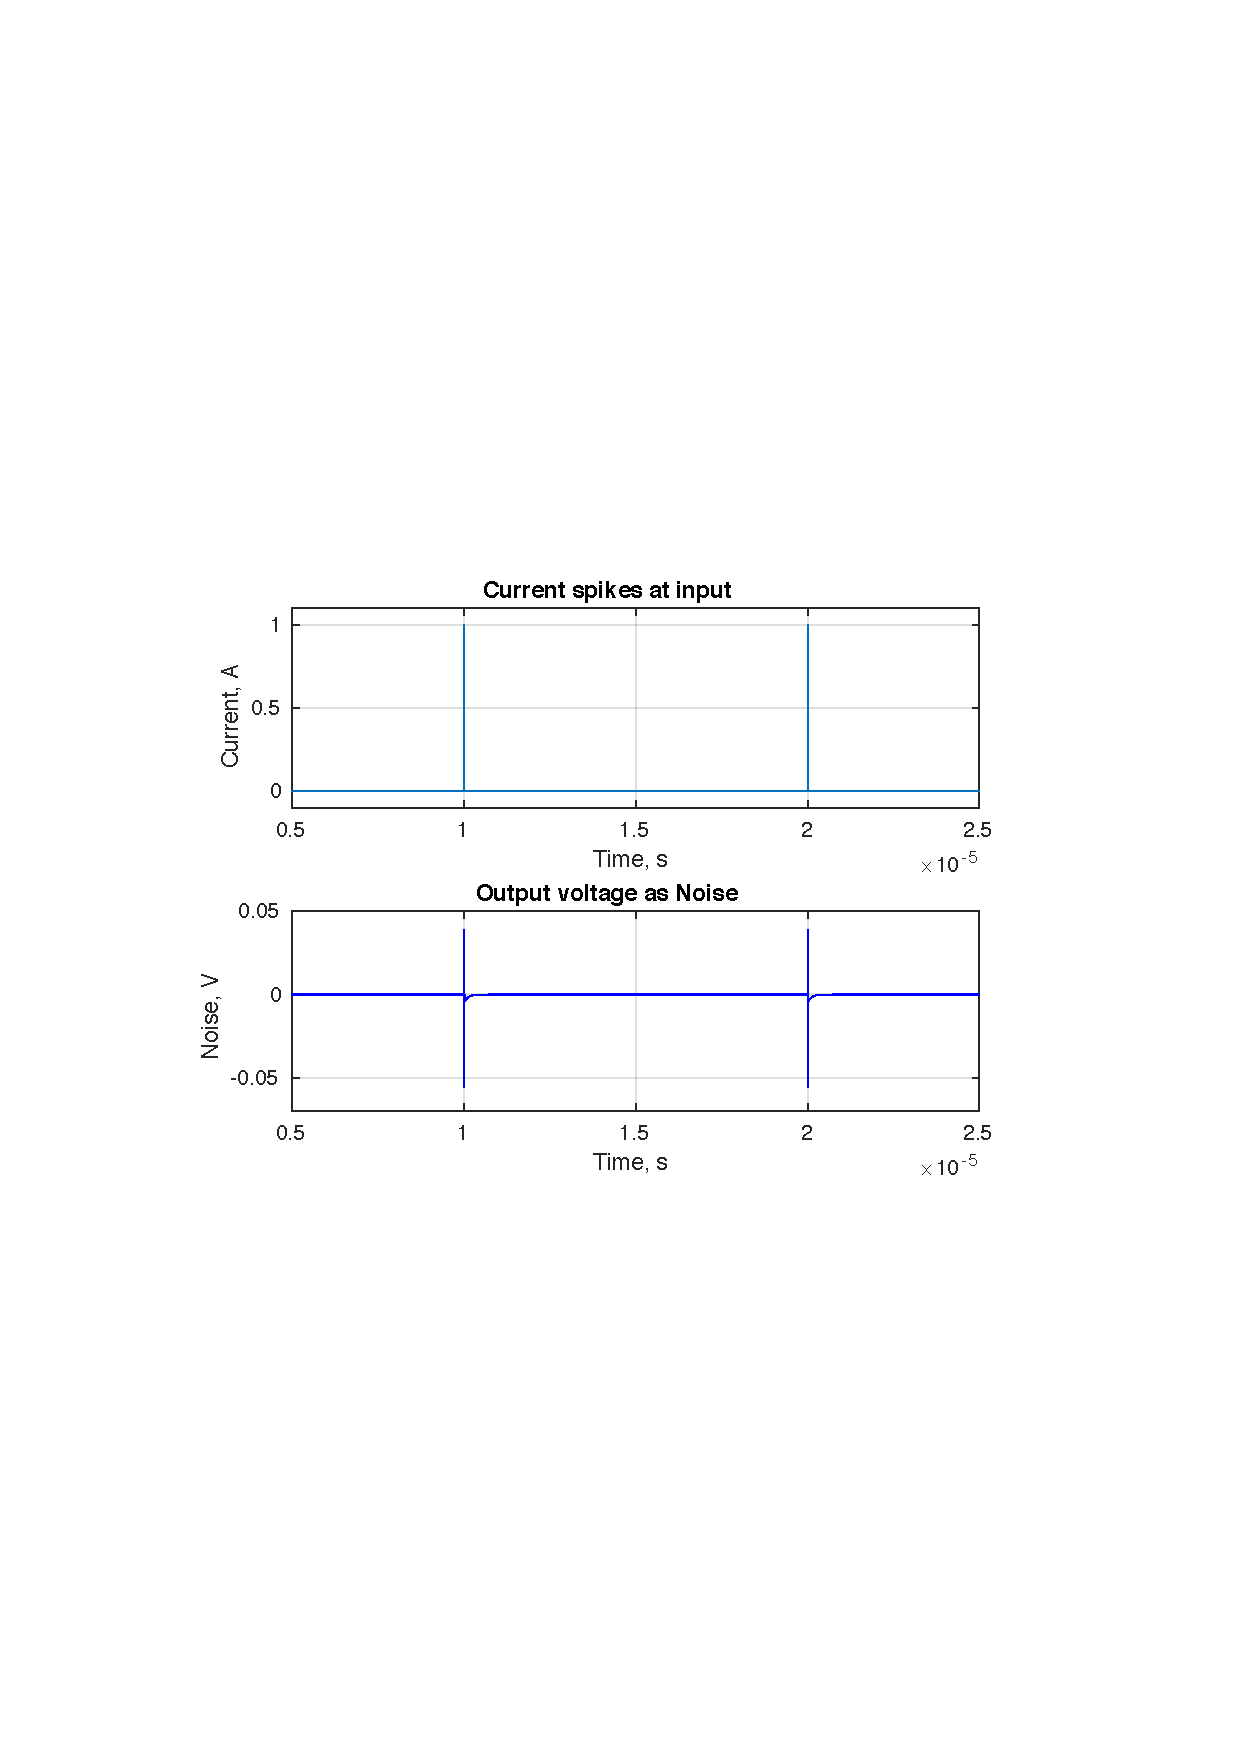
\includegraphics[width=0.95\textwidth]{img/3e_tran.pdf} 
  \caption{Current spikes input and voltage noise output}
  \label{cap_tran} 
\end{figure}

\begin{figure} [H]
  \centering 
  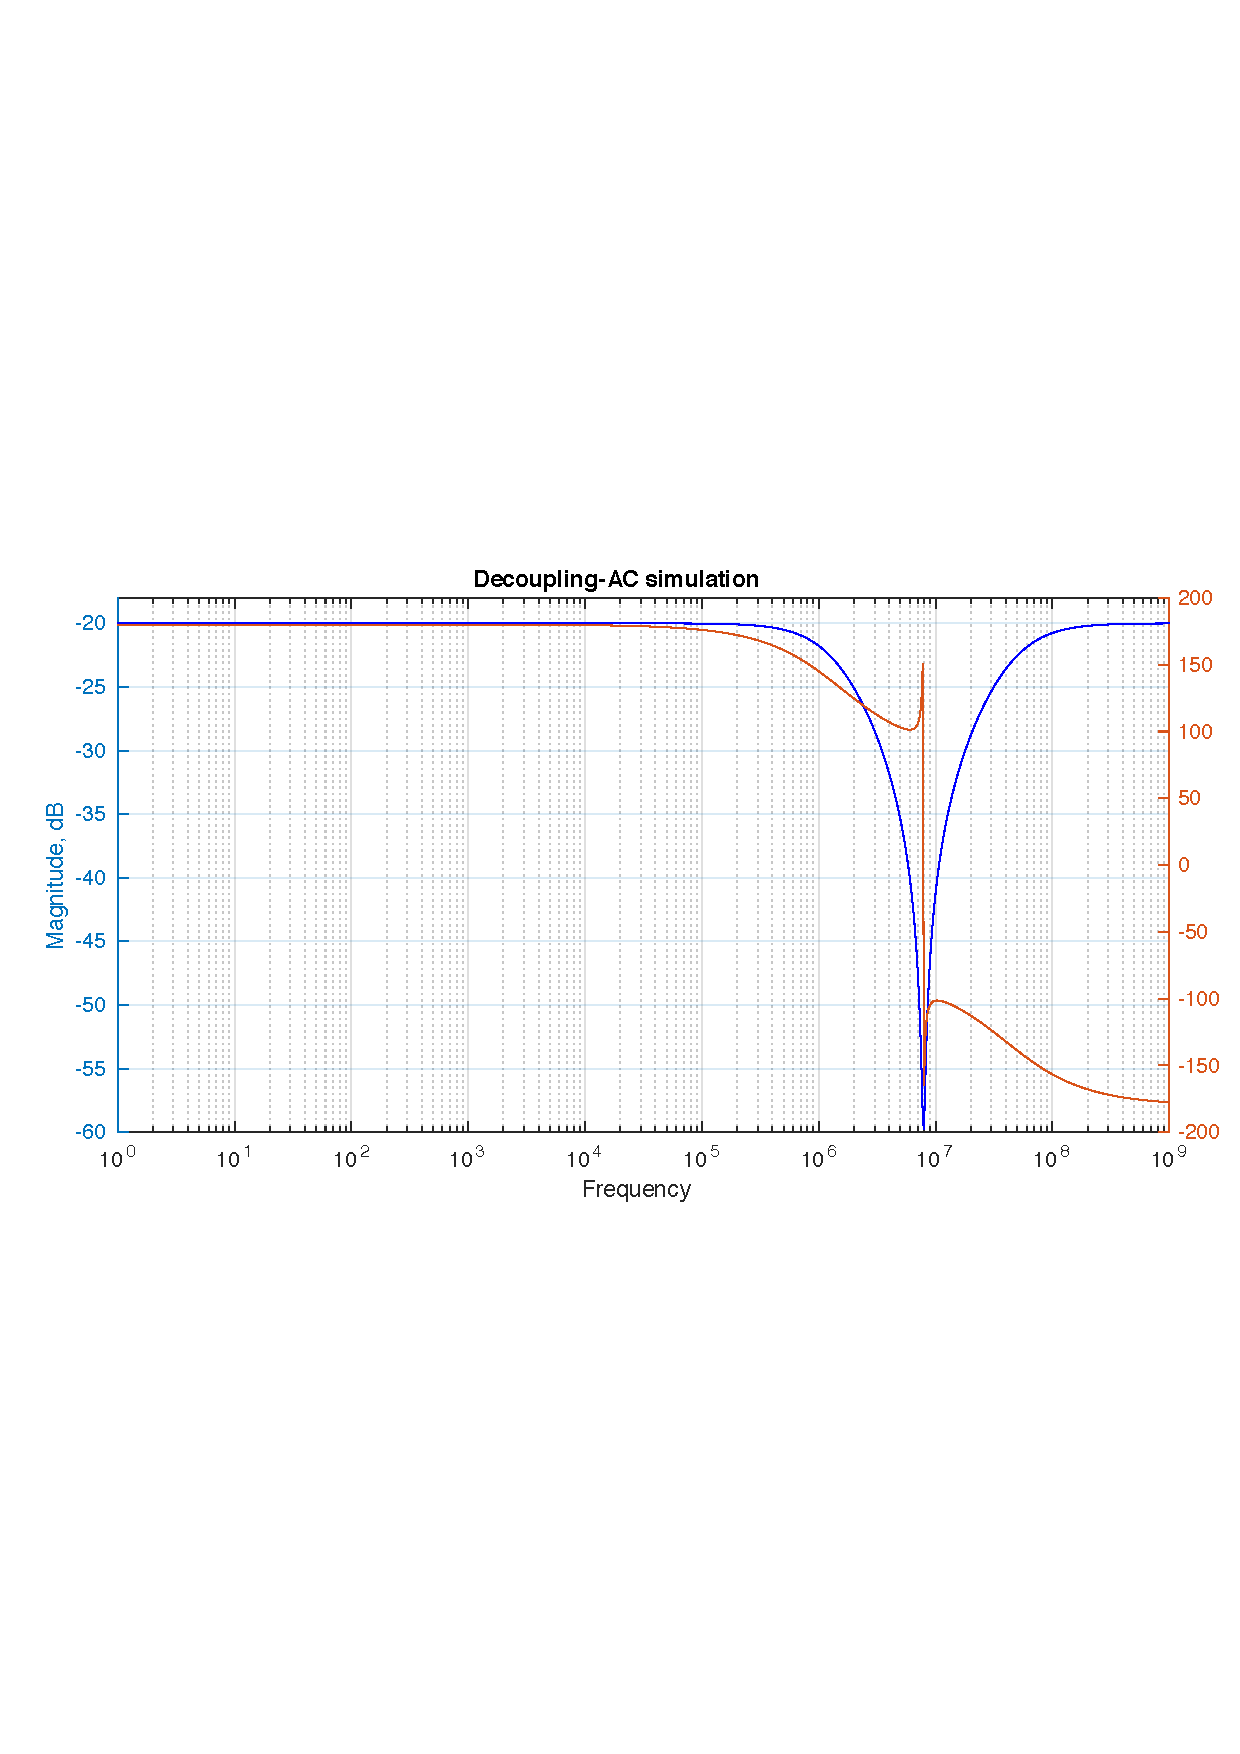
\includegraphics[width=\textwidth]{img/3e_ac.pdf} 
  \caption{AC analysis of decoupled output}
  \label{cap_ac} 
\end{figure}

%% Task 3f
\subsection{}
Figure  \ref{cap_tran2} and  \ref{cap_ac2}  are transient and frequency simulation results with comparison between different Tr and Tf. The difference is seen only in the time domain because in spite of different rise and fall time, both the signal have same frequency and hence magnitude and phase are unaffected. 

In case of transient signal in figure \ref{cap_tran2}, it can be noticed that the voltage spikes due to the input current spikes of shorter Tr and Tf exceed our stability requirement. The spikes are close to 0.095 V whereas the requirement is to reduce it below 0.075 V.
\begin{figure} [H]
  \centering 
  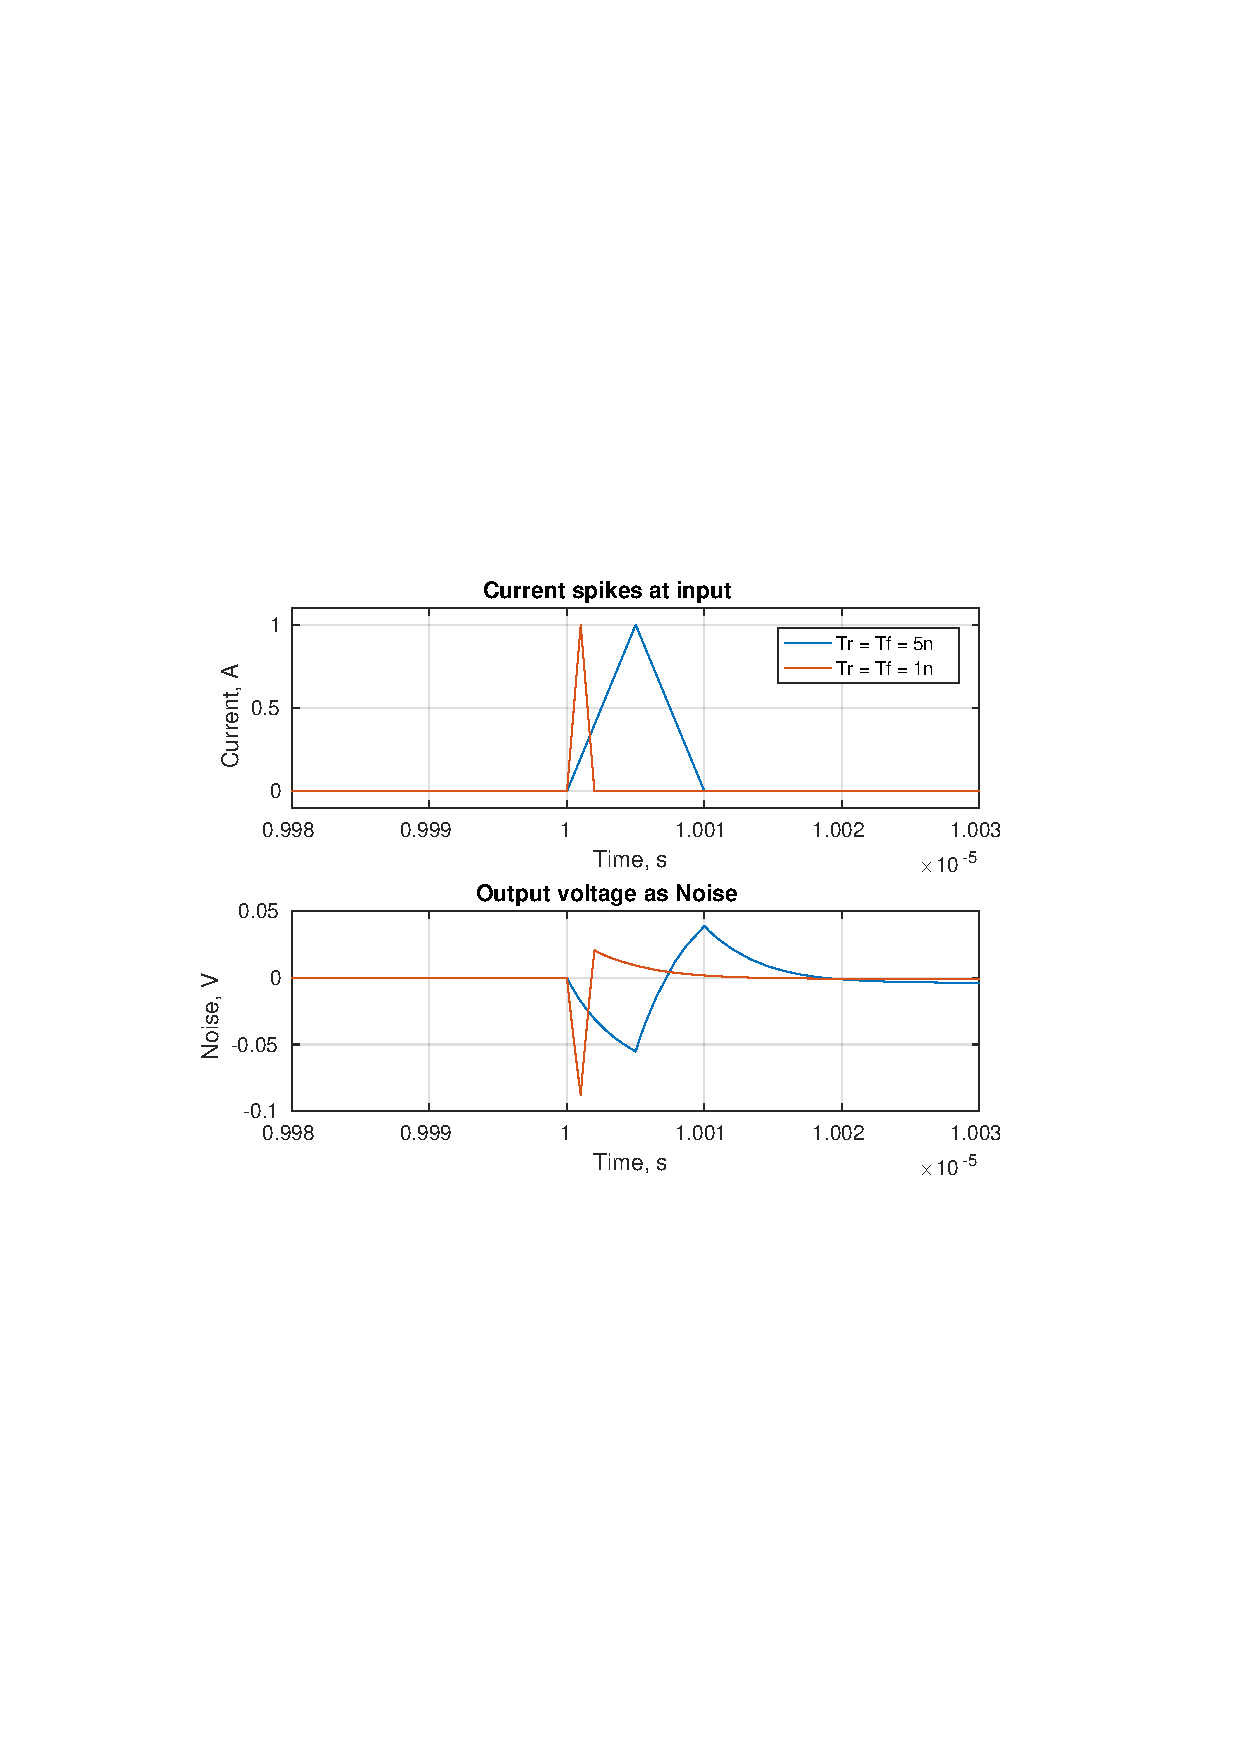
\includegraphics[width=0.85\textwidth]{img/3f_tran.pdf} 
  \caption{Current spikes with shorter Tr and Tf and voltage output as noise}
  \label{cap_tran2} 
\end{figure}

\begin{figure} [H]
  \centering 
  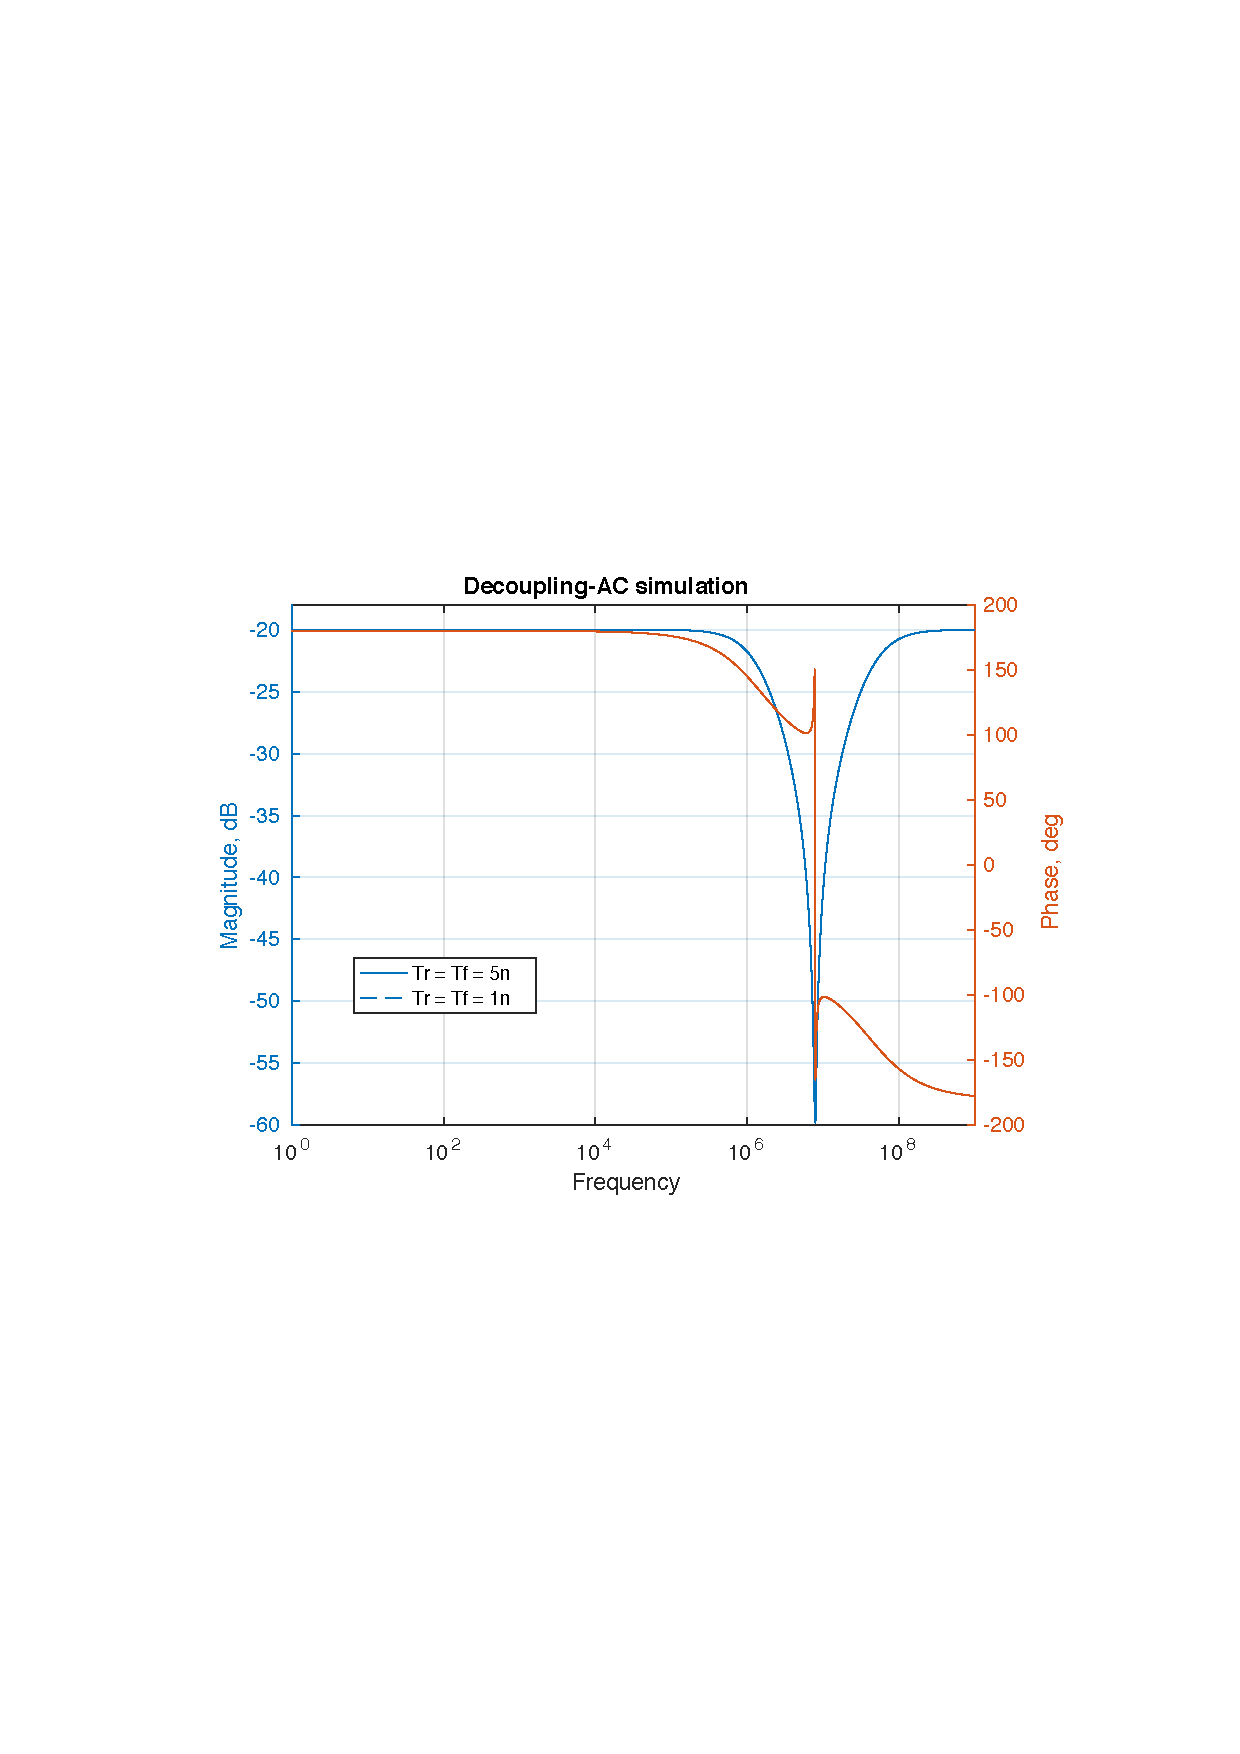
\includegraphics[width=0.85\textwidth]{img/3f_ac.pdf} 
  \caption{AC of decoupled output noise with different Tr and Tf}
  \label{cap_ac2} 
\end{figure}

%% Task 4
\section{Parasitic capacitive coupling}
%% Task 4a
\subsection{Noise captured}
Figure \ref{two_con} is the two parallel conductors both of length 10 cm. The parasitic capacitance between the lines is 0.1 pF/cm. Conductor 1 carry a signal of 5 V swing and conductor 2 has a capacitor and resistor in parallel to ground of 10 pF and $10 M\Omega$. To the right of  figure \ref{two_con} illustrates the equivalent parasitic coupling in terms of lumped capacitors, also shown in figure  \ref{sch_4a} . 


\begin{figure} [H]
  \centering 
  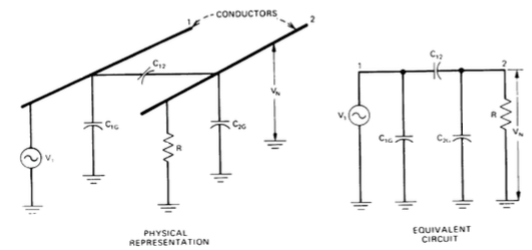
\includegraphics[width=0.9\textwidth]{img/two_con.png} 
  \caption{Capacitive coupling between two conductors}
  \label{two_con} 
\end{figure}

\begin{figure} [H]
  \centering 
  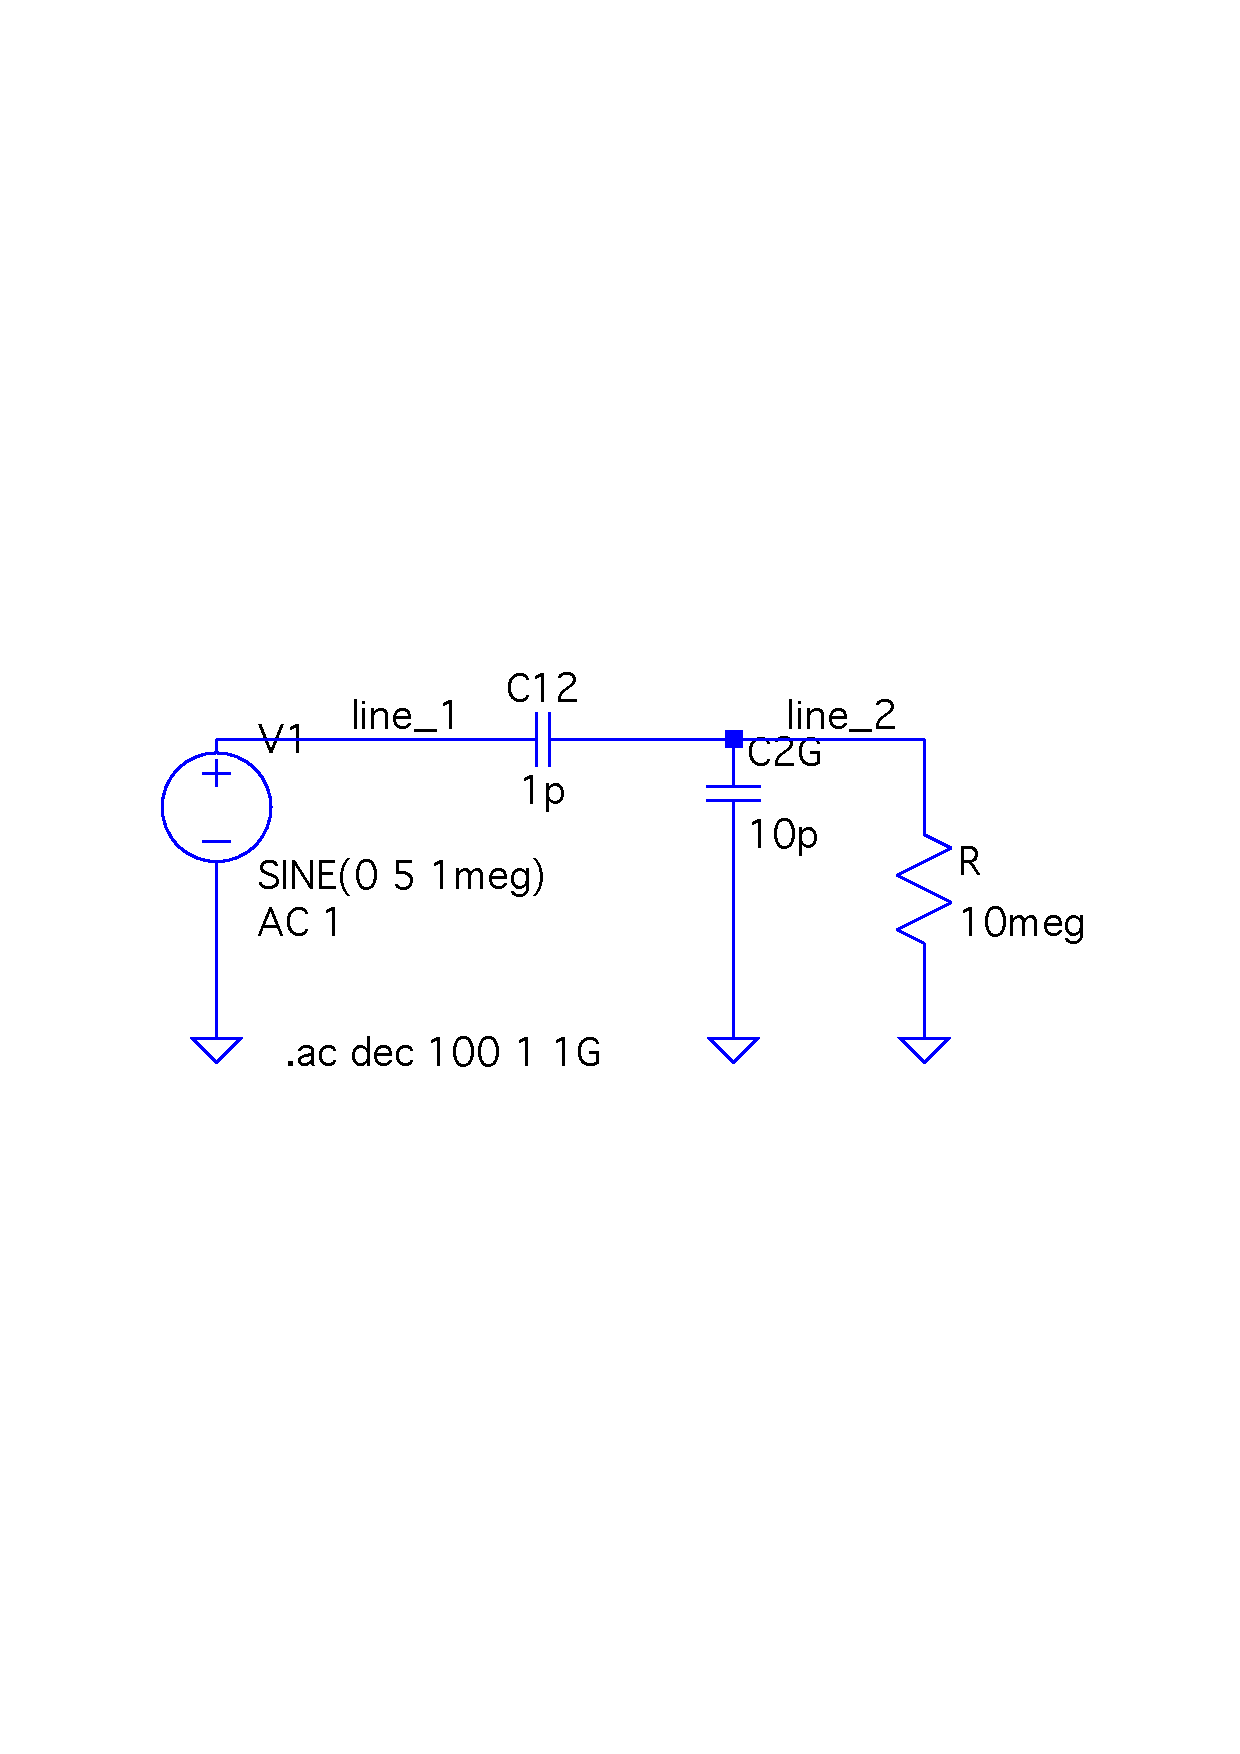
\includegraphics[width=0.9\textwidth]{img/sch_4a.pdf} 
  \caption{Schematic of capacitive coupling between two conductors}
  \label{sch_4a} 
\end{figure}



Similarly  \ref{two_con_sh} shows the same two conductors where conductor 2 is shield. To the right is its equivalent circuit which is also shown is figure  \ref{sch_4b}. Here $C_{12}$ is parasitic between conductor 1 and 2, which is 1pF without shield. $C_{2G}$ is capacitor between conductor 2 and ground. R is a resistor connected between conductor 2 and ground. $C_{2S}$ is parasitic between conductor 2 and shield which is 1 pF/cm. 

In presence of shield, $C_{12}$ decreases. If L be the length of shield, then
\begin{equation*}
C_{12} =  1 pF - 0.1pF/cm * L
\end{equation*}

Similarly with shield, $C_{12}$ increases as 
\begin{equation*}
C_{2S} =  1 pF * L
\end{equation*}

Whereas, $C_{2G}$ being a physical component remains the same.

The worst case noise magnitude is given as below which is used for calculation. This is valid when shield does not cover all the length of the conductor. When there is no shield, we take
$C_{2S} = 0$.
\begin{equation*}
V_N = \frac{C_{12}}{C_{12}+C_{2G}+C_{2S}}   
\end{equation*}


\begin{figure} [H]
  \centering 
  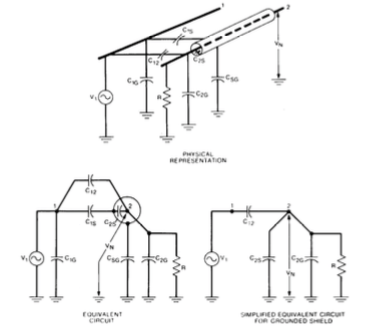
\includegraphics[width=0.9\textwidth]{img/two_con_sh.png} 
  \caption{Capacitive coupling between two conductors with shielding}
  \label{two_con_sh} 
\end{figure}

\begin{figure} [H]
  \centering 
  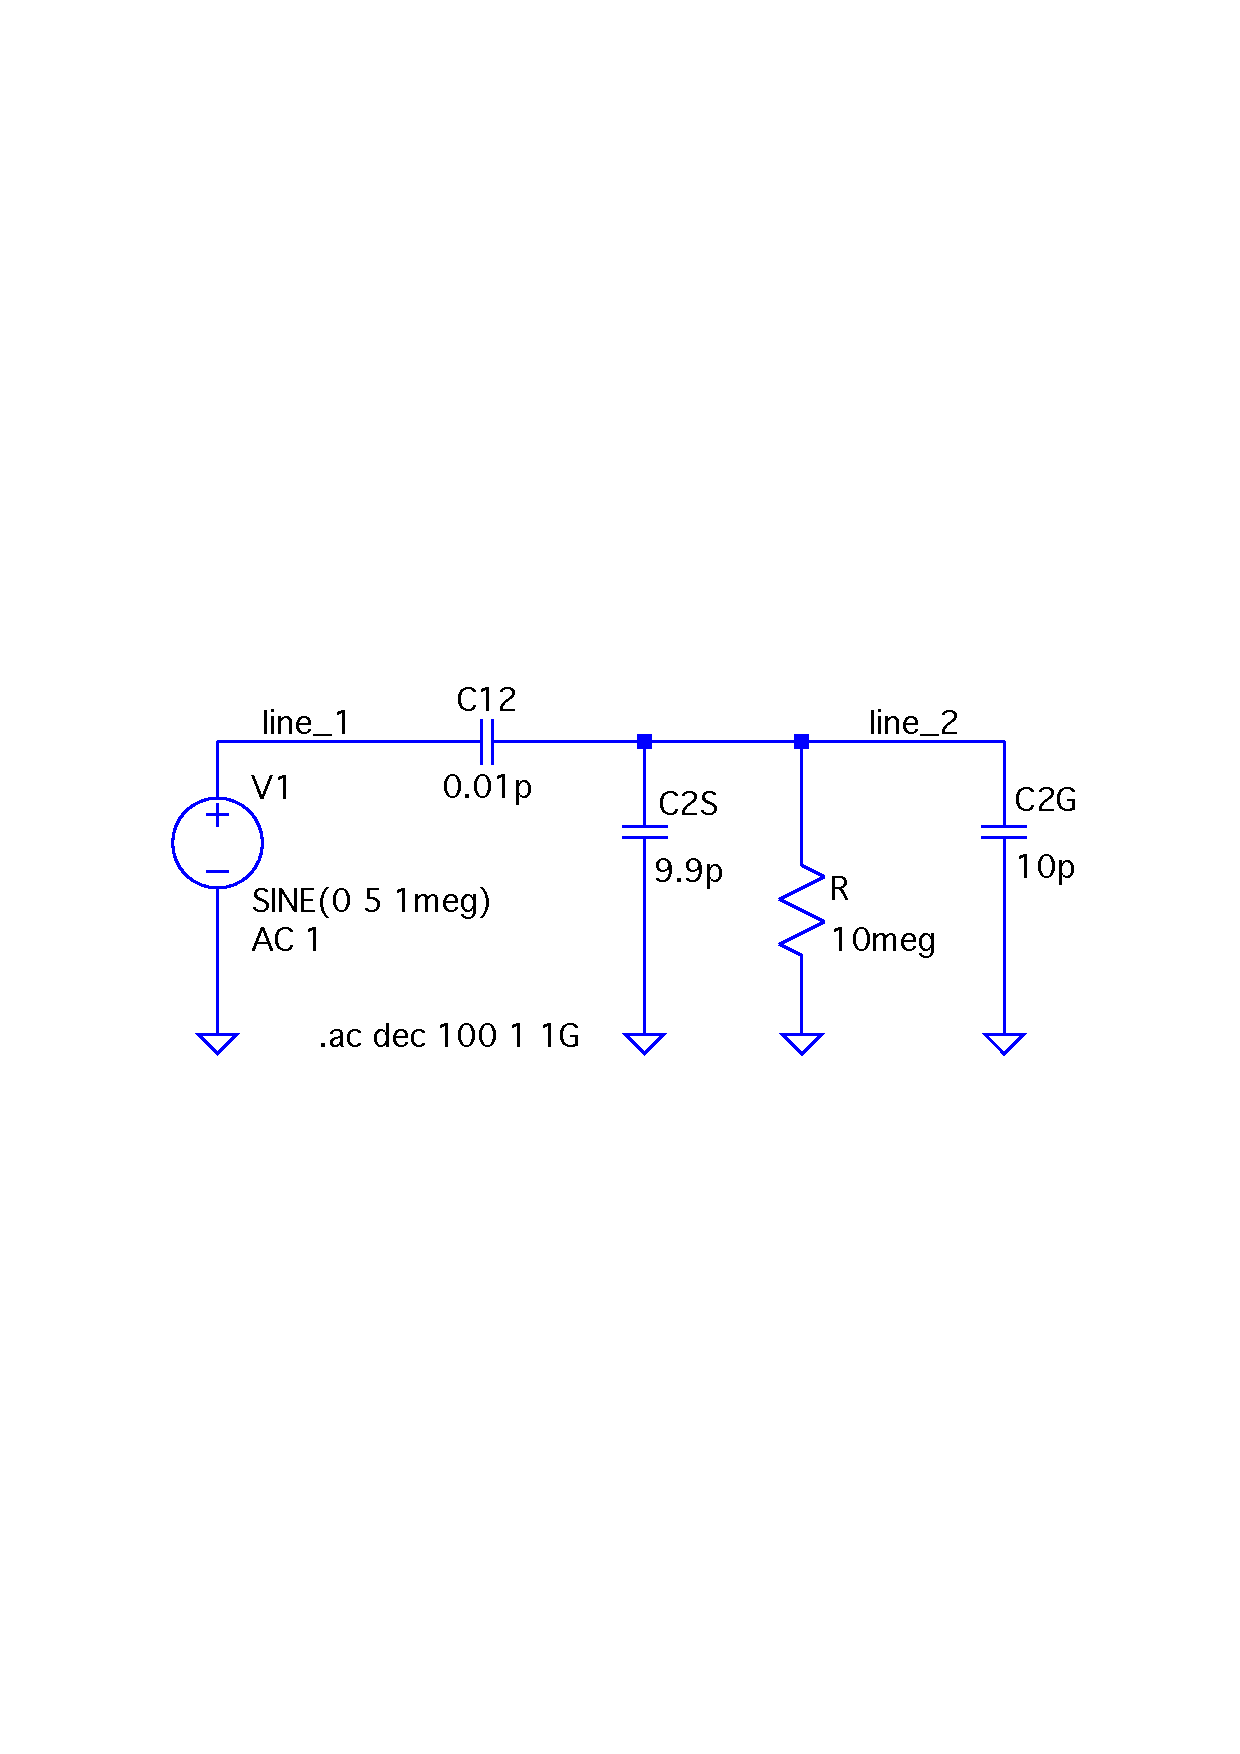
\includegraphics[width=\textwidth]{img/sch_4b.pdf} 
  \caption{Schematic of capacitive coupling between two conductors with shielding}
  \label{sch_4b} 
\end{figure}

Noise received by conductor 2 with shield of varying length and without shield is analysed. Table \ref{noise} summarises the calculated values and   \ref{two_con_ac} shows the simulated frequency response.
\begin{table}[H]
\caption{Parasitic capacitance and shielding}
\begin{center}
\begin{tabular}{c|c|c|c|c}
\hline \hline
L  (cm) & $C_{12} (pF)$ & $C_{2S} (pF)$ & $C_{2G} (pF)$ & Noise (dB) calculated\\ \hline
0  & 1 & 0 & 10 & -20.8 \\ \hline
2  & 0.8 & 2 & 10 & -24.1\\ \hline
5  & 0.5 & 5  & 10 & -29.8 \\ \hline
9  & 0.1 & 9  & 10 &-45.6\\ \hline
9.9  & 0.01 & 9.9 & 10 &-66\\ 
\hline \hline
\end{tabular}
\end{center}
\label{noise}
\end{table}%


\begin{figure} [H]
  \centering 
  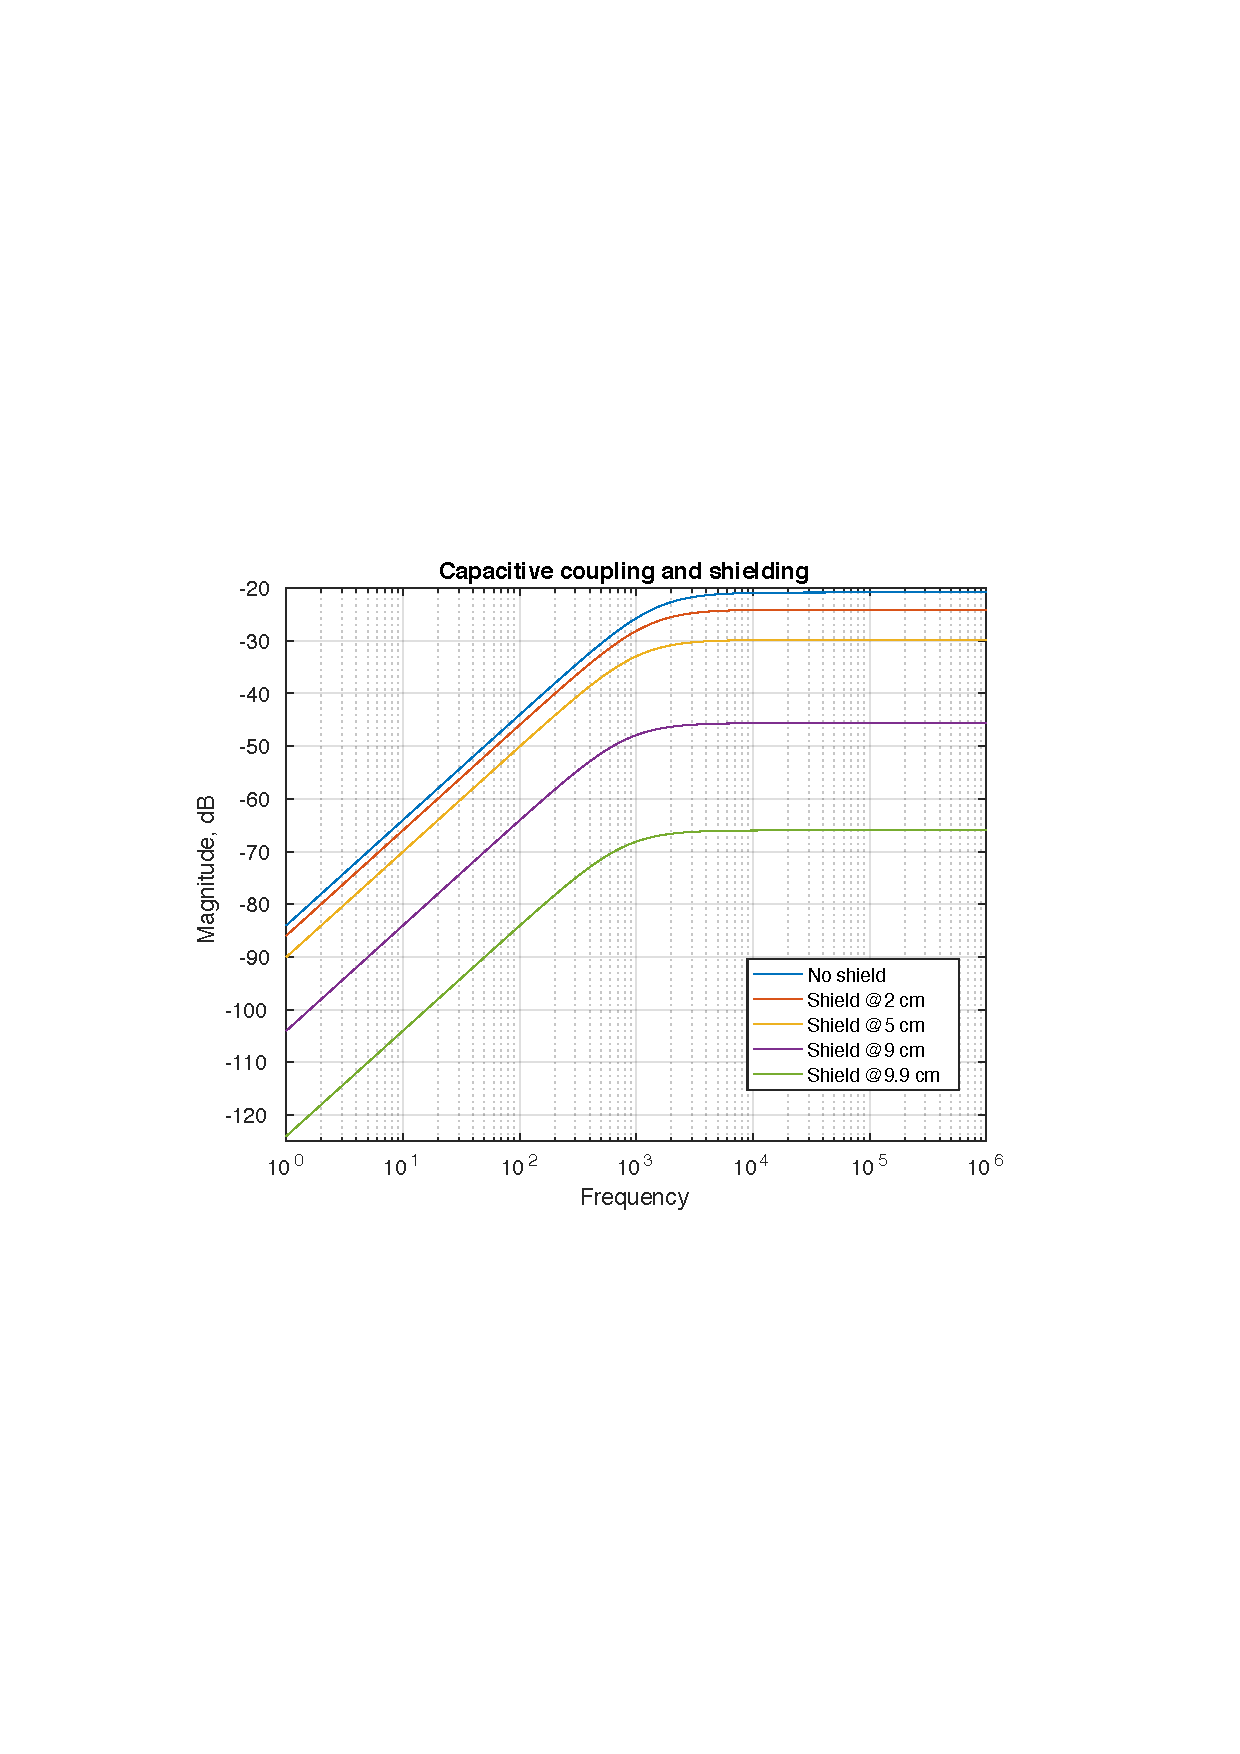
\includegraphics[width=1\textwidth]{img/4.pdf} 
  \caption{Frequency response of capacitive coupled noise voltage}
  \label{two_con_ac} 
\end{figure}

From figure \ref{two_con_ac} and table \ref{noise}, it is seen that simulated and calculated magnitude of noise is almost the same .Both shows that capacitive coupling decreases with increase in length of shield and hence the noise picked by conductor two. The plot also shows that corner frequency has decreased too.

\section{Artificial source of transient analysis}
%%task 5a
\subsection{BV sources}
 Figure \ref{sch_5a} is the schematics of two BV sources and WH1 and WH2 in figure \ref{bv_white} are white noises generated using those sources in LTspice using WHITE function with same index. Since the subtracted noise in the last plot below is zero for all time, it looks like WHITE generate the same random value for same index and hence it cannot be considered as true white noise.

\begin{figure} [H]
  \centering 
  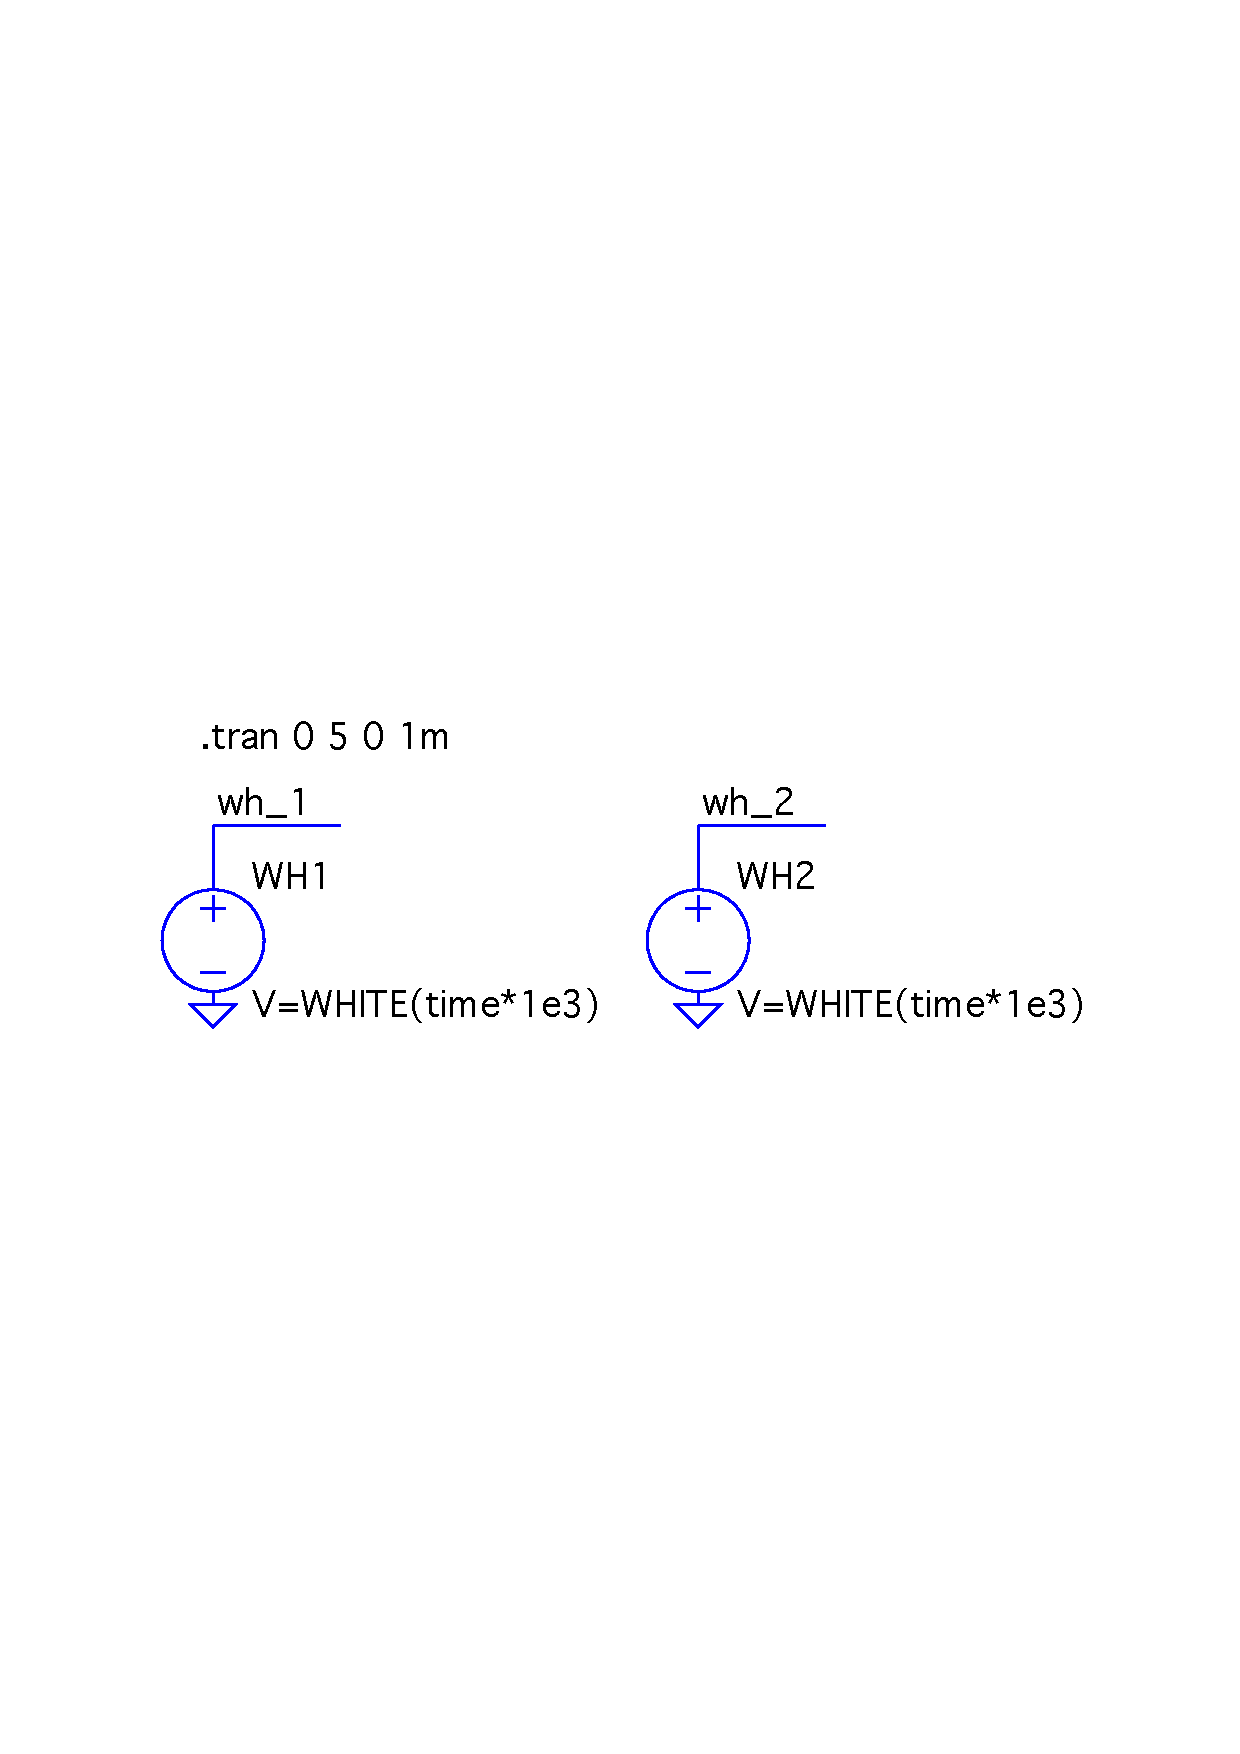
\includegraphics[width=0.9\textwidth]{img/sch_5a.pdf} 
  \caption{Schematics of BV white noise}
  \label{sch_5a} 
\end{figure}

\begin{figure} [H]
  \centering 
  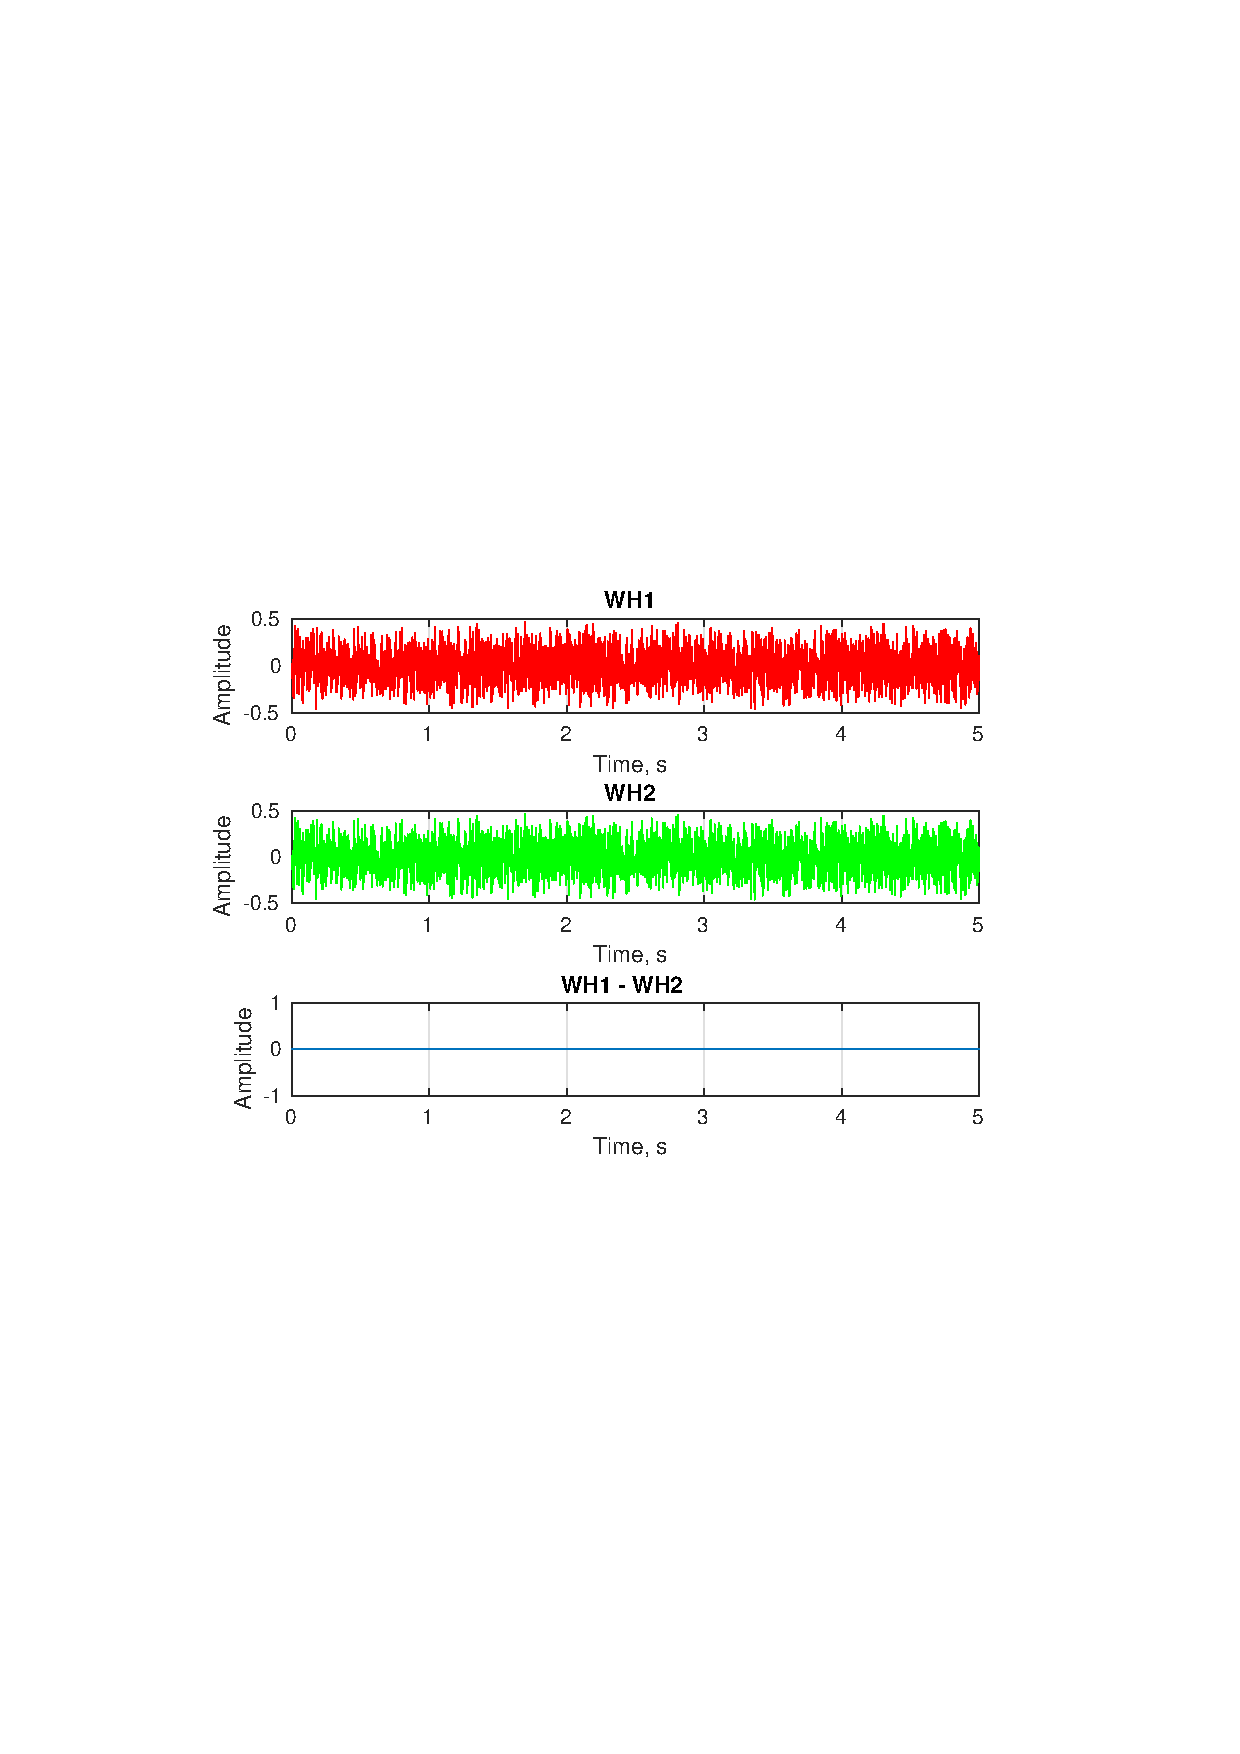
\includegraphics[width=0.9\textwidth]{img/5a.pdf} 
  \caption{White noise from BV sources}
  \label{bv_white} 
\end{figure}
%% task 5b
\subsection{BV sources with different time index}
 Figure \ref{bv_white2} again illustrates the white noises from BV sources where WH2 is changed by 1. The subtraction of WH1 and WH2 is now neither zero nor constant, hence looks like these may be considered white noises. The amplitude is still within -0.5 to +0.5. The truth is white noise has a normal distribution and WH1 and WH2 distribution is not normal. 
 
\begin{figure} [H]
  \centering 
  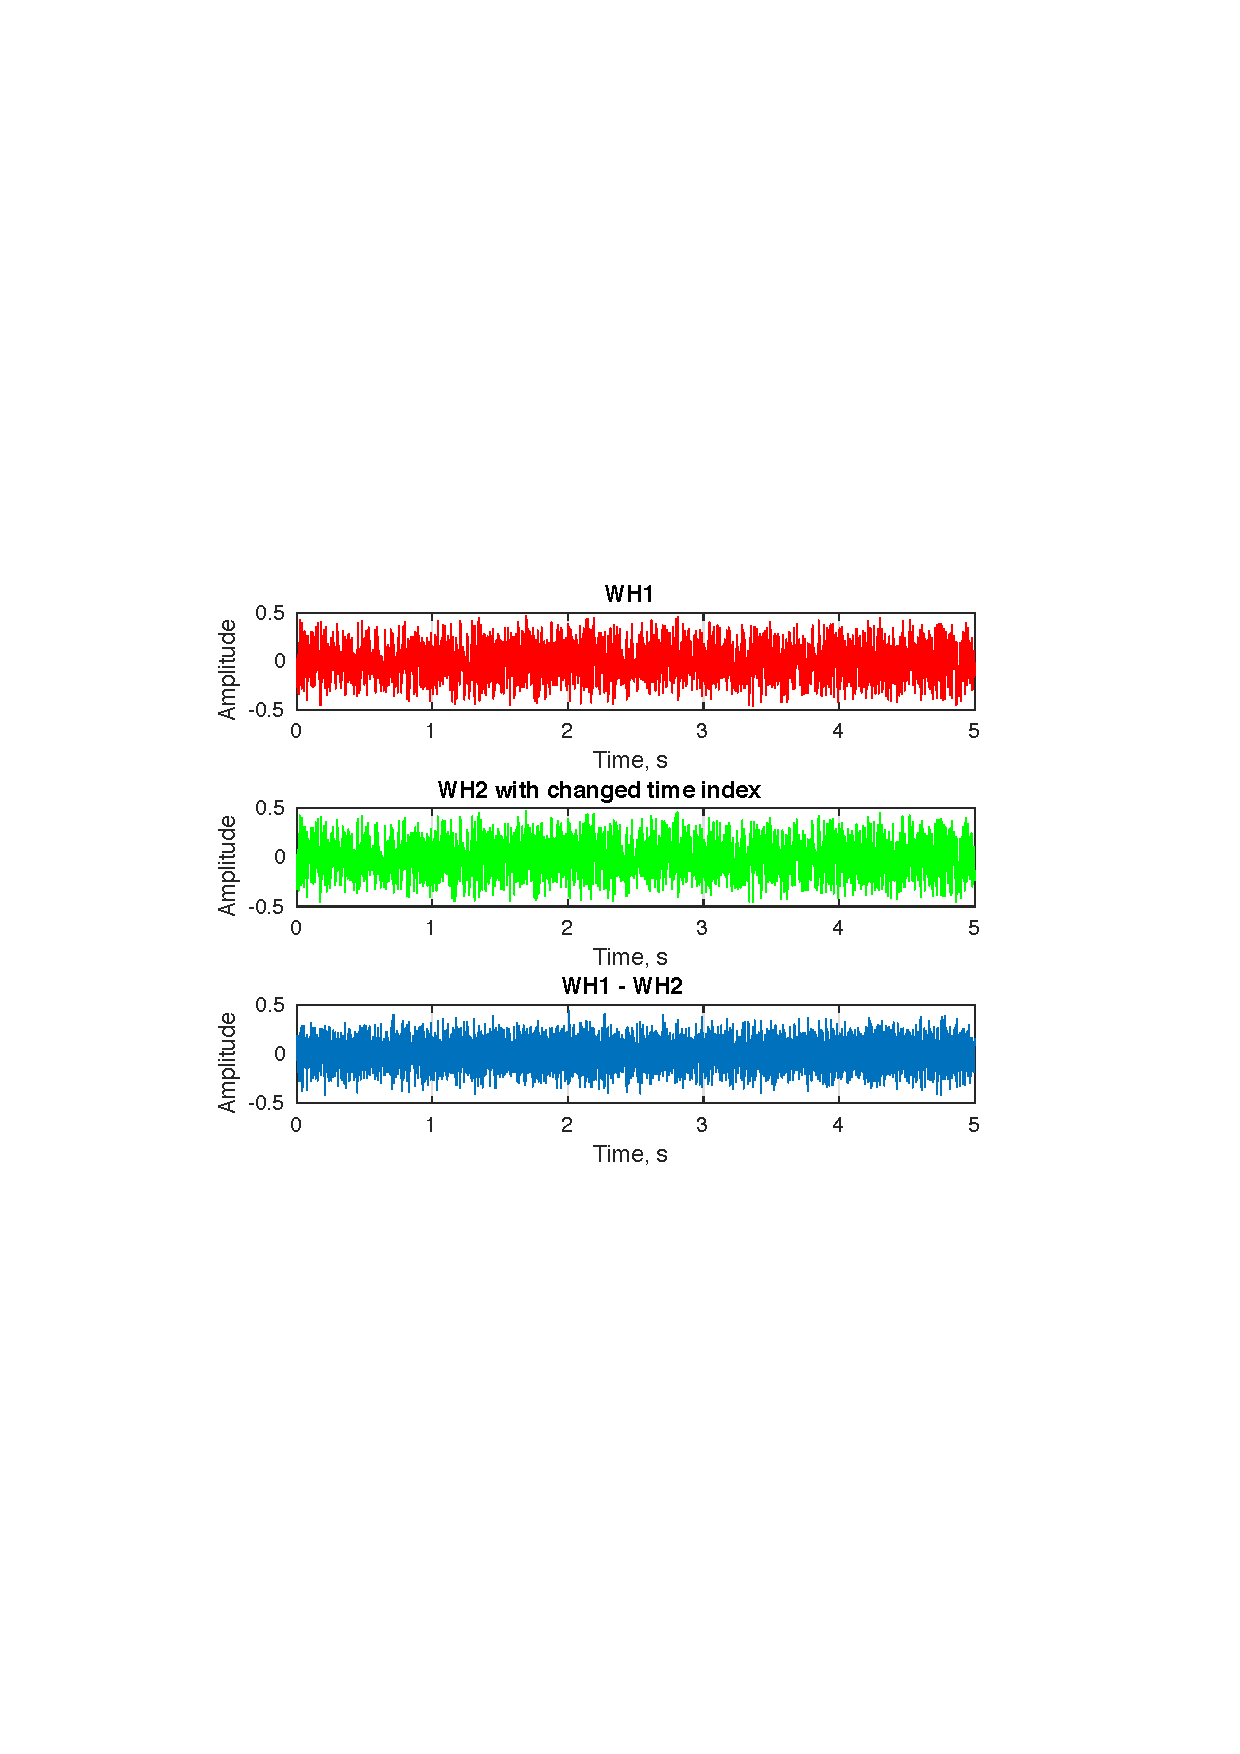
\includegraphics[width=0.9\textwidth]{img/5b.pdf} 
  \caption{White noise from BV sources with different time index}
  \label{bv_white2} 
\end{figure}
%%Task 5c
\subsection{Noise from file and BV source}
Figure \ref{white3} is the comparison of noise generated from provided file and BV source. The FILE1 has larger amplitude and looks more normal whereas WH1 from BV source has smaller magnitude. The difference between these too looks even more random with some spikes grater in amplitude than FILE1. The schematic is shown in  \ref{sch_5c}. 

\begin{figure} [H]
  \centering 
  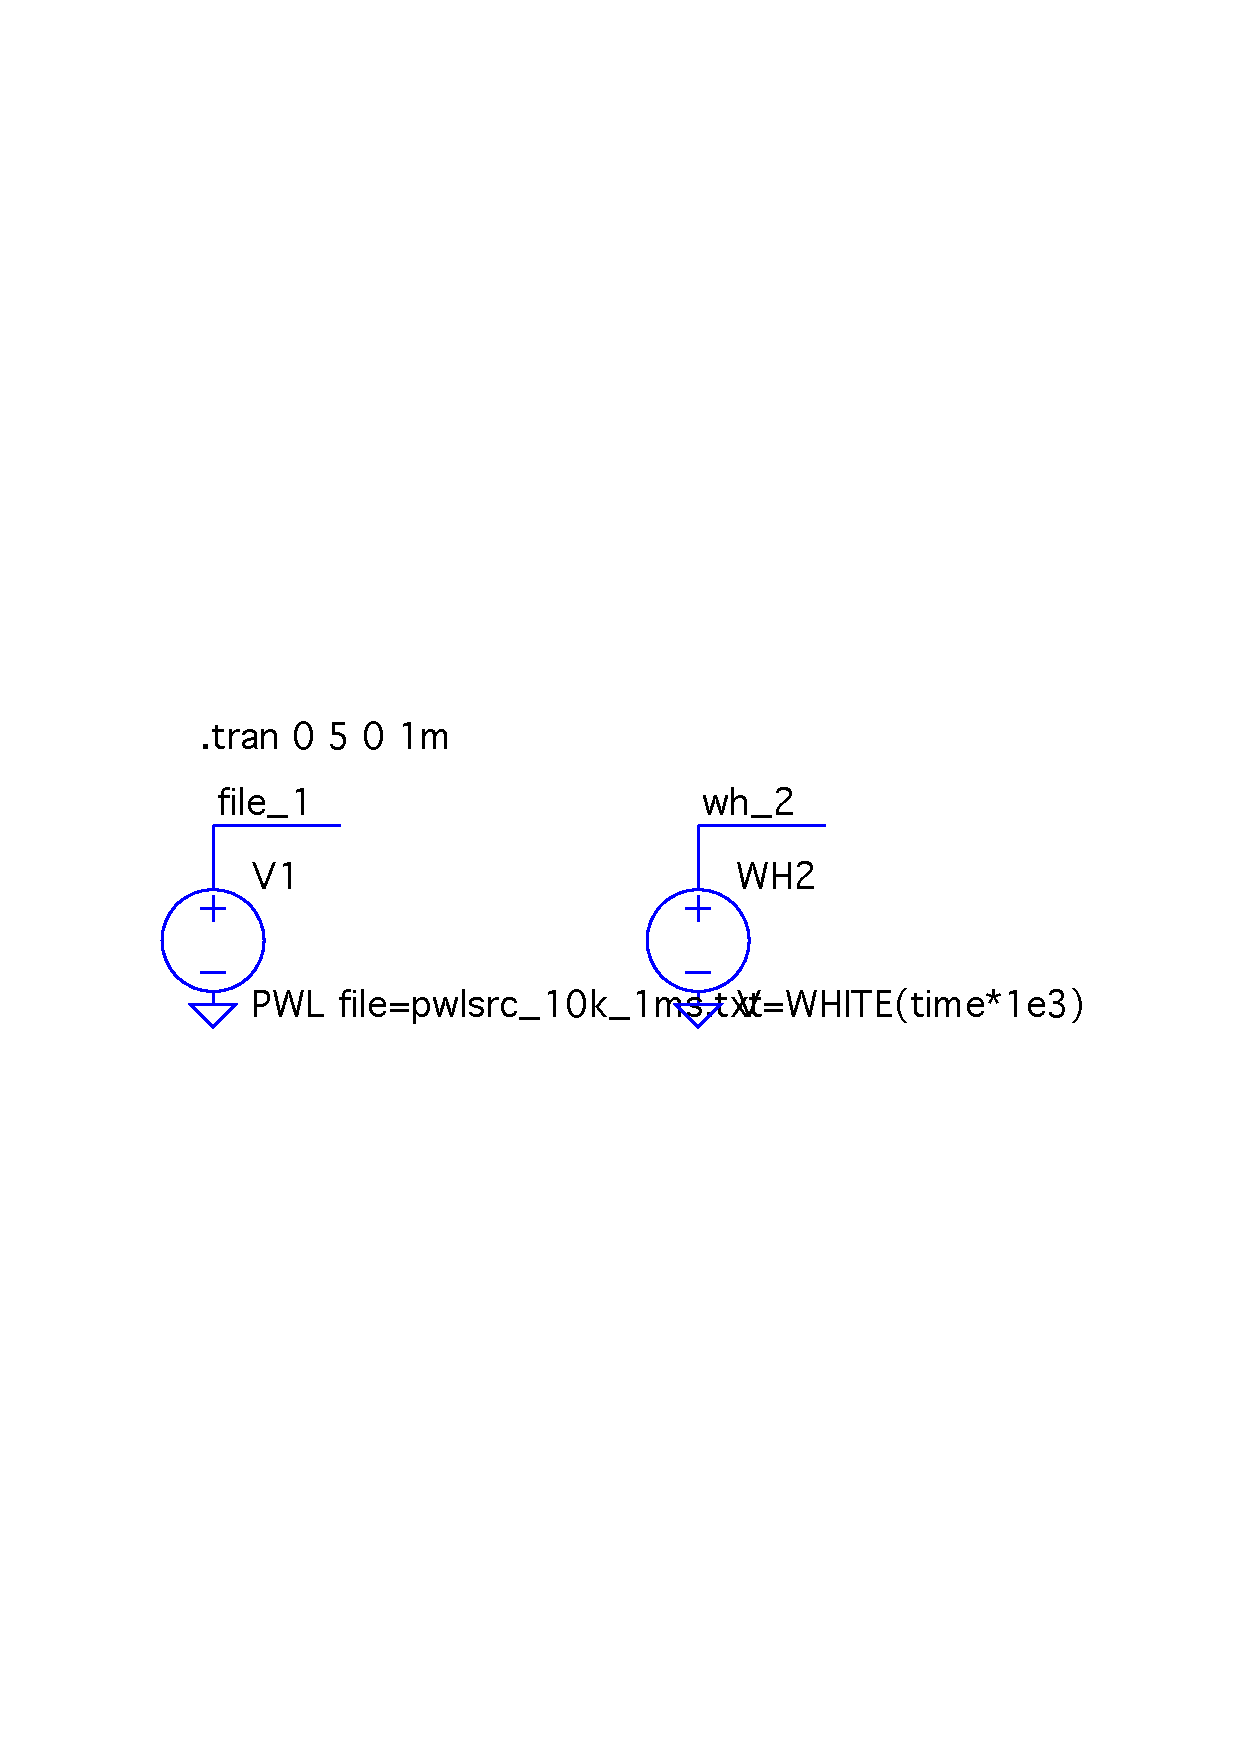
\includegraphics[width=0.9\textwidth]{img/sch_5c.pdf} 
  \caption{Schematic of file noise source and BV source}
  \label{sch_5c} 
\end{figure}

\begin{figure} [H]
  \centering 
  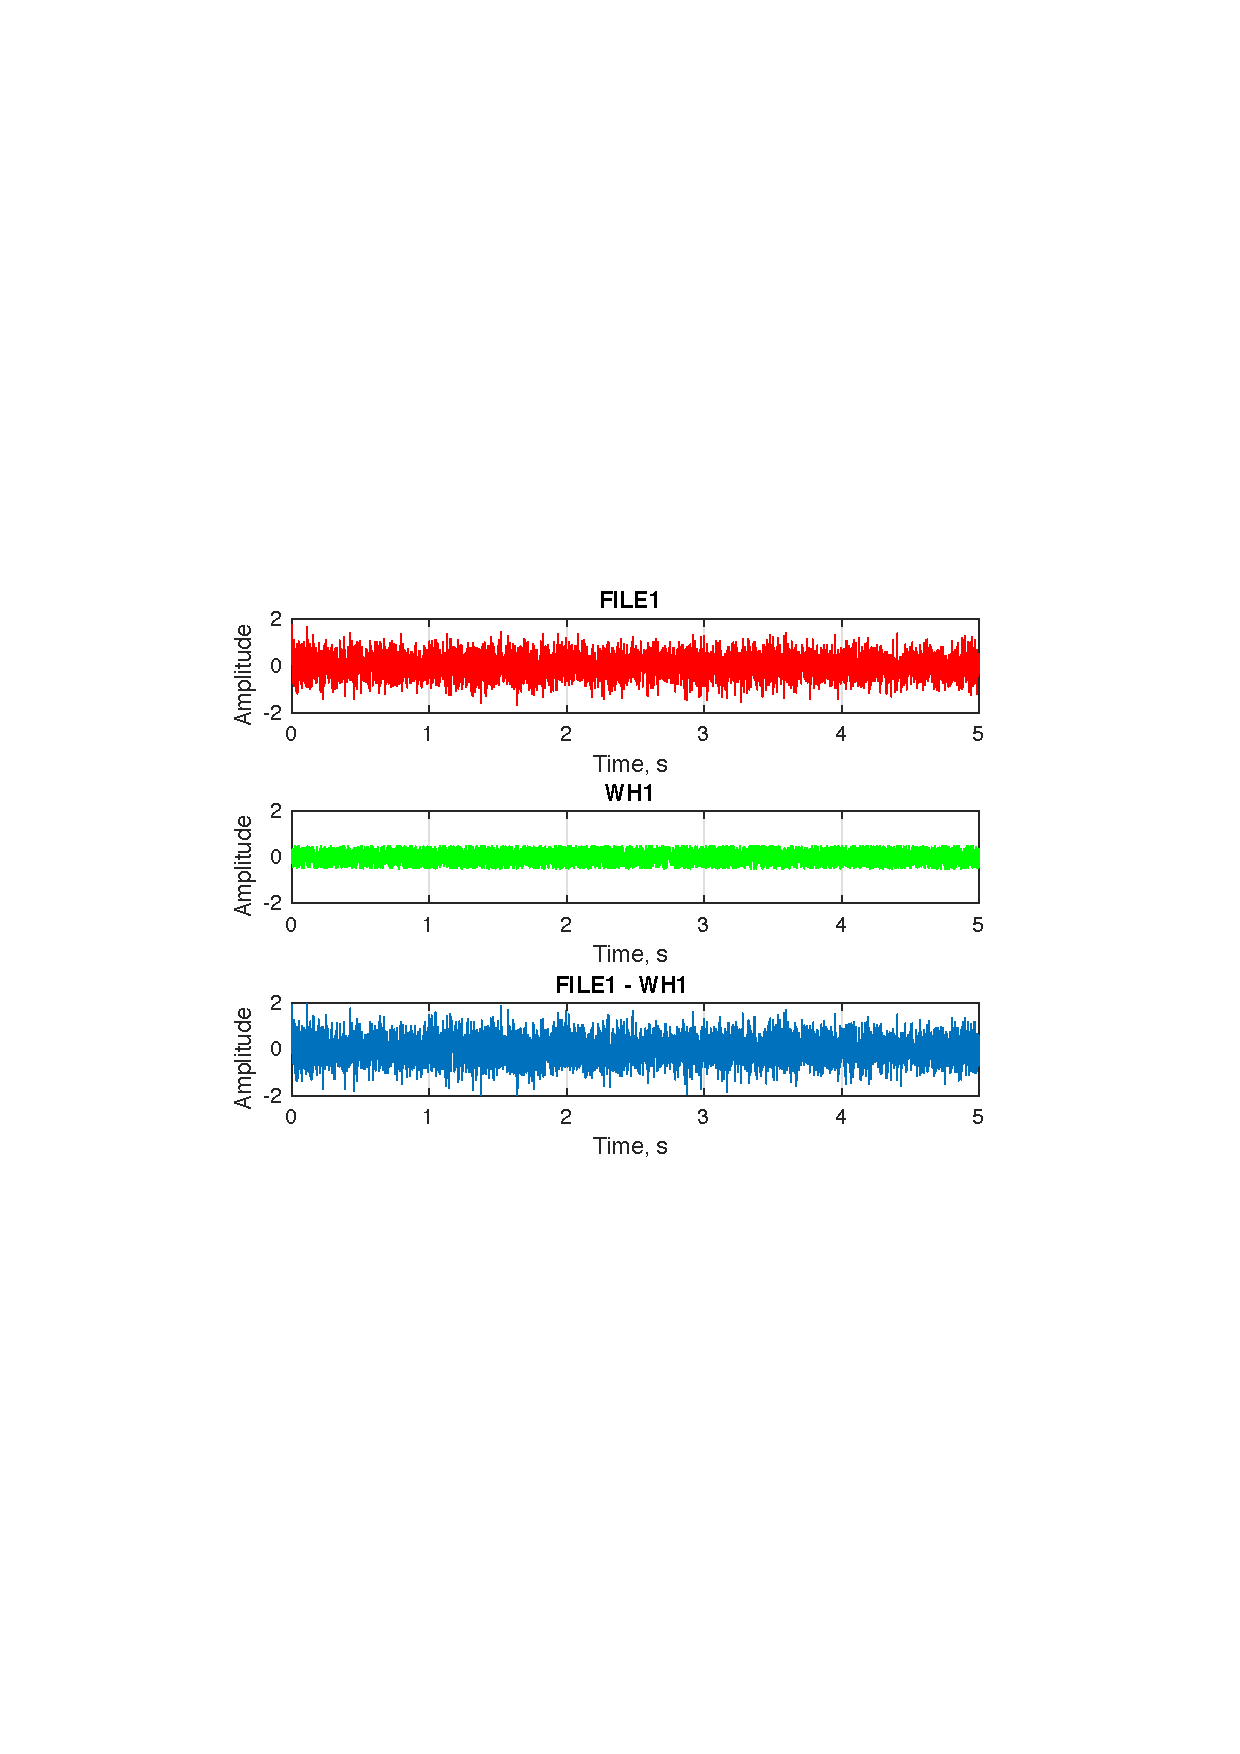
\includegraphics[width=0.9\textwidth]{img/5c.pdf} 
  \caption{Noise from file and BV}
  \label{white3} 
\end{figure}

\subsection{FILE1 and delayed FILE1}
 Figure \ref{white4} illustrates noise from file, FILE1 and FILE2 which is delayed FILE1 by 1 ms. The set up as shown in \ref{sch_5d} The difference in these signal looks like even more random with some spikes going beyond 2 V. It seems like the distribution is still normal with increase in deviation. 
 \begin{figure} [H]
  \centering 
  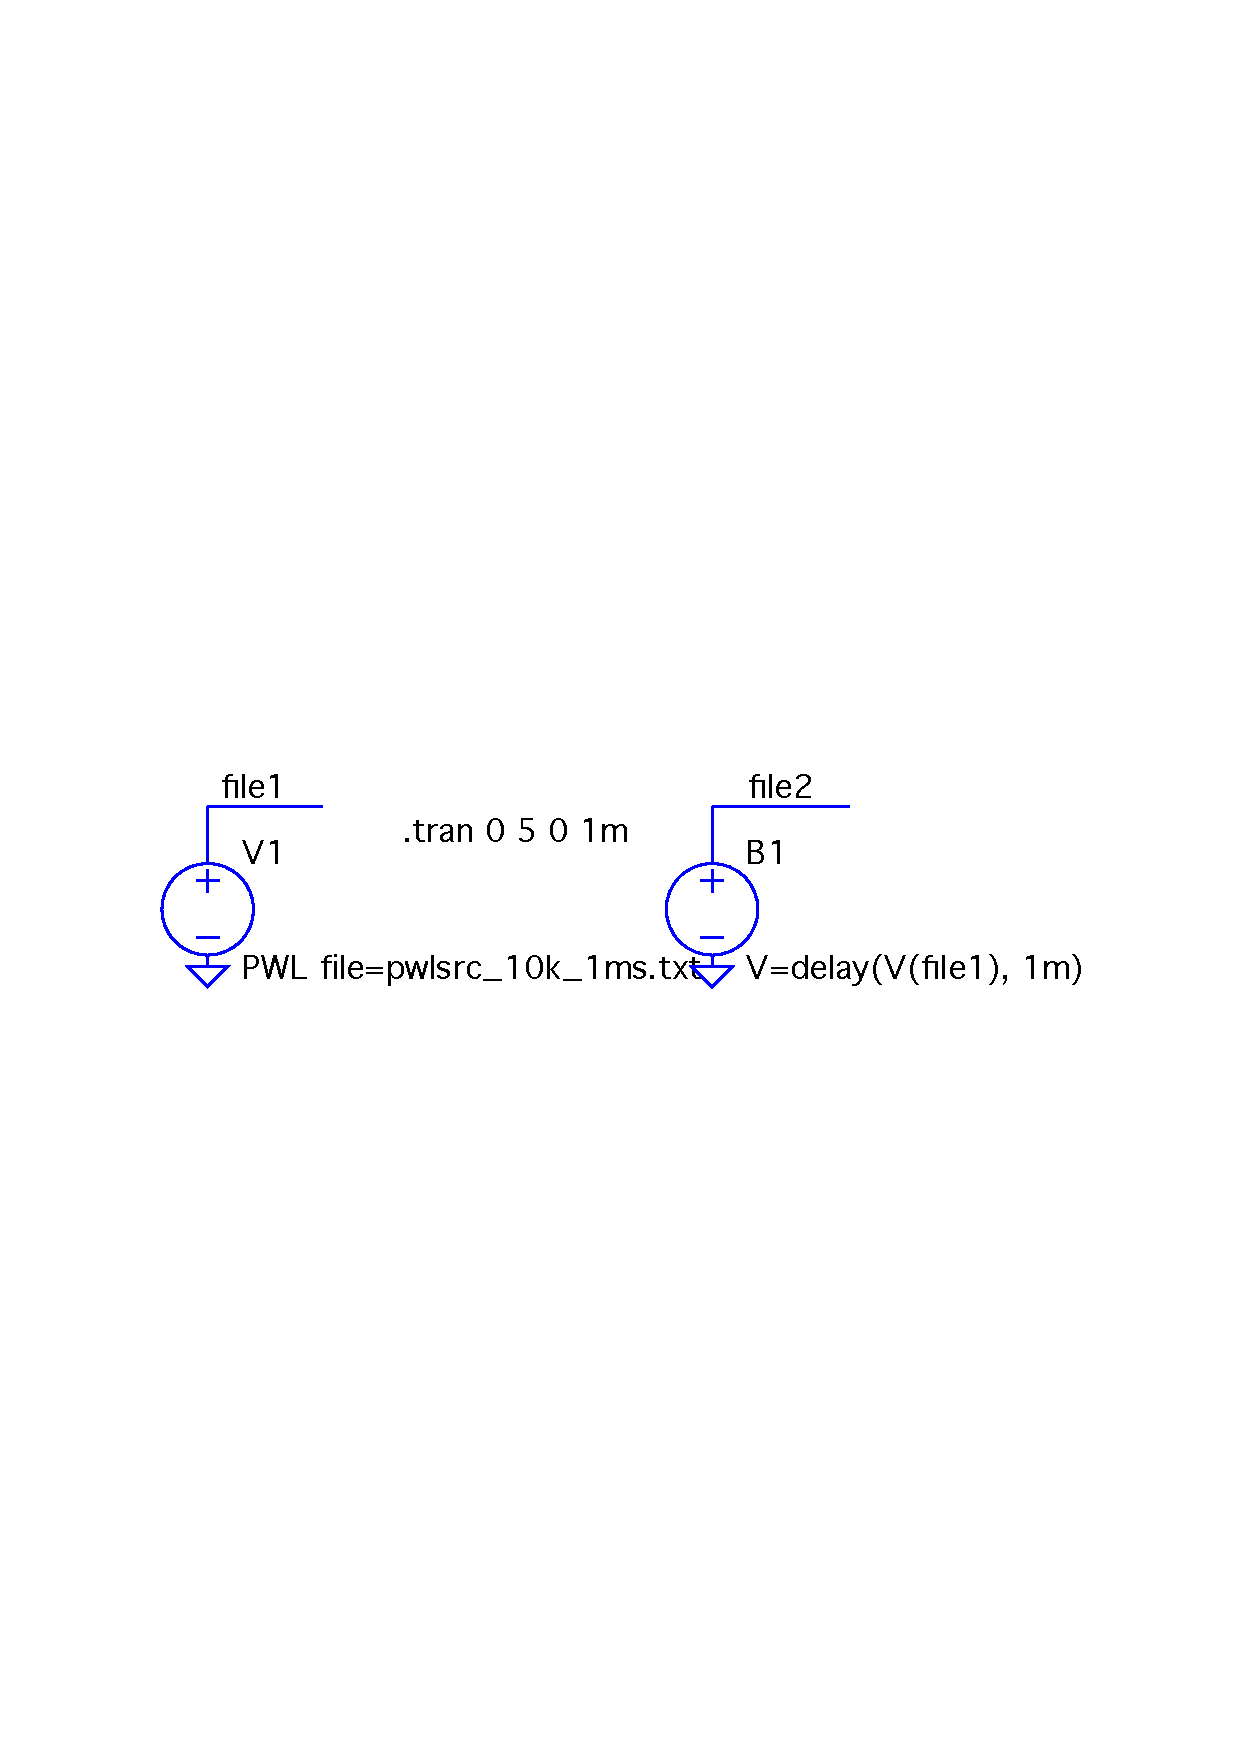
\includegraphics[width=0.9\textwidth]{img/sch_5d.pdf} 
  \caption{Schematic set up of file noise and its delay}
  \label{sch_5d} 
\end{figure}

 
\begin{figure} [H]
  \centering 
  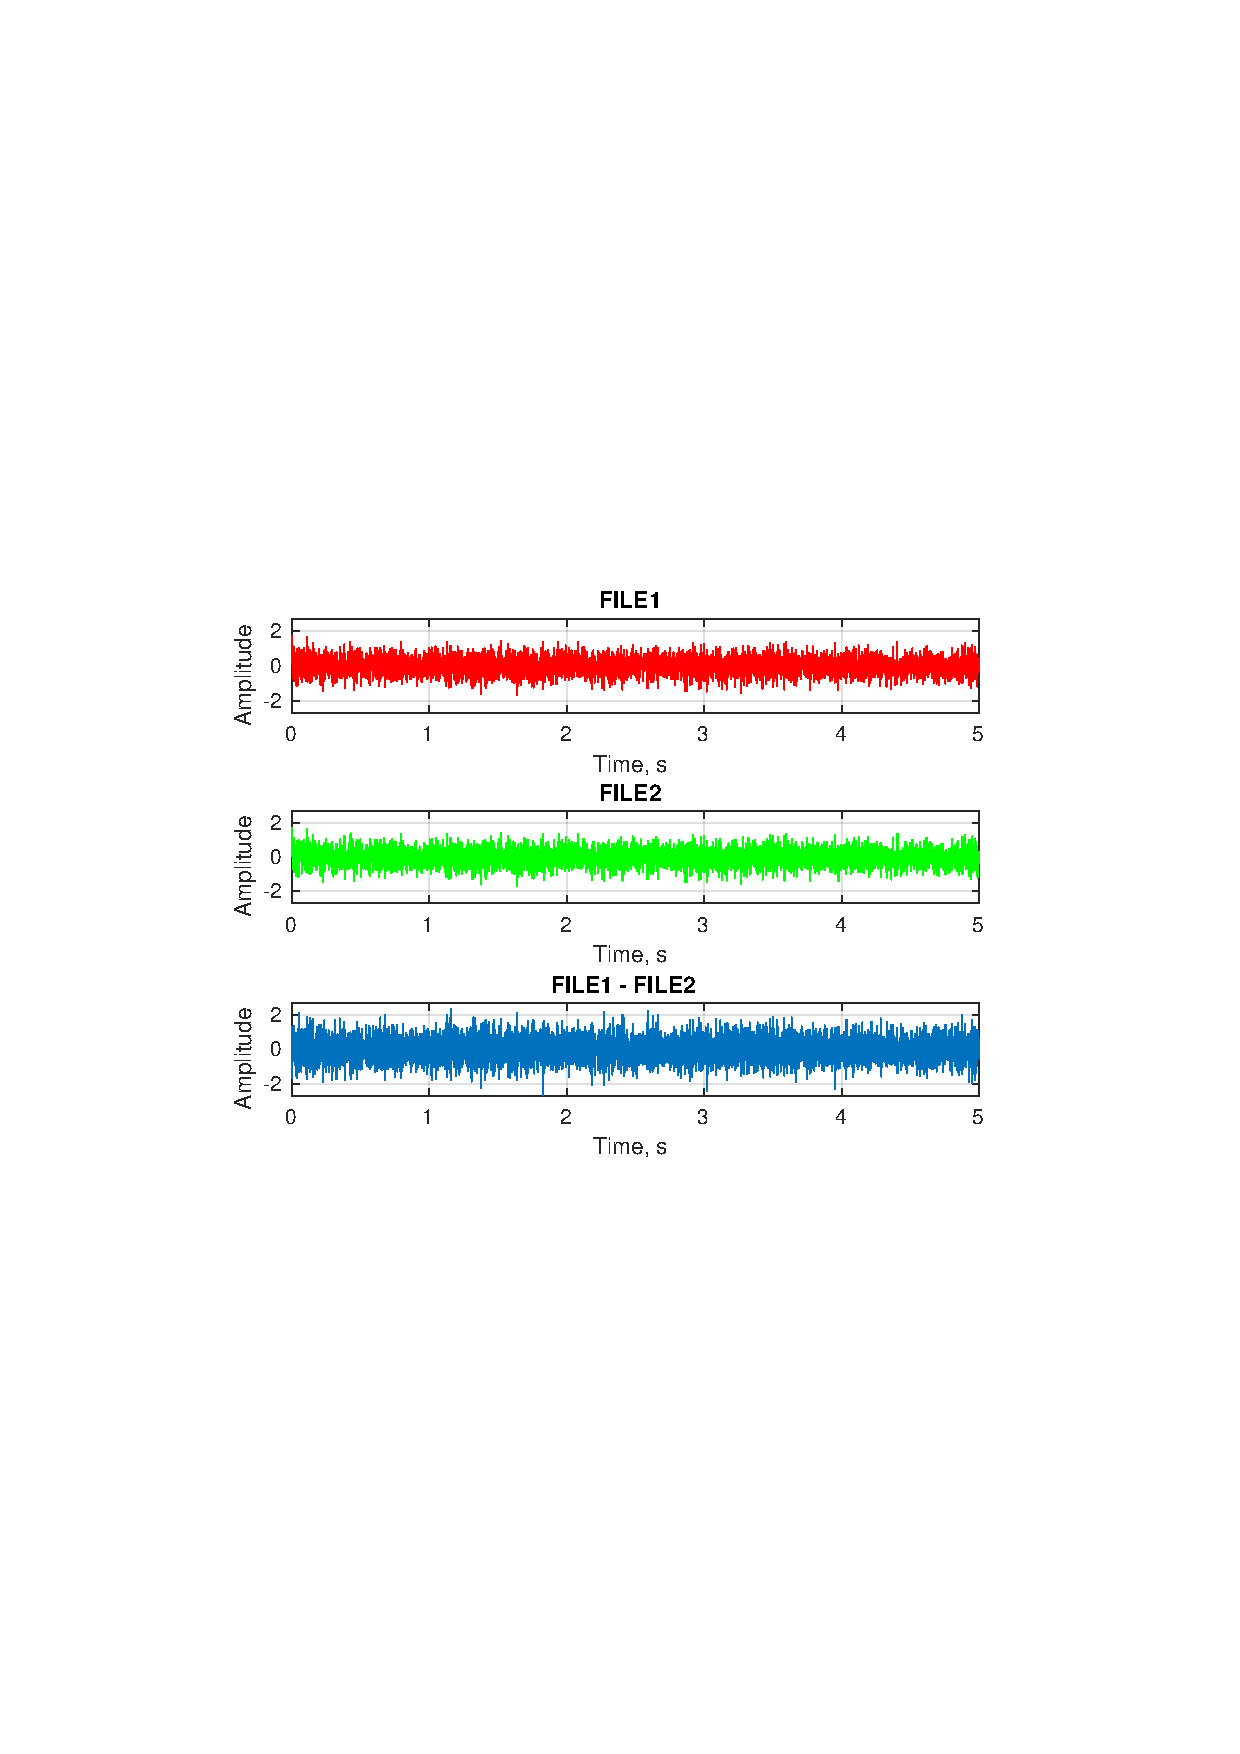
\includegraphics[width=0.9\textwidth]{img/5d.pdf} 
  \caption{FILE1 and delayed FILE1}
  \label{white4} 
\end{figure}

\end{document}
